\documentclass[11pt,a4paper]{ctexart}
\usepackage[toc]{multitoc}%目录两栏
\usepackage{mathrsfs}
\usepackage{color}
\usepackage{titlesec}
\usepackage{amsmath,amsthm,amssymb}
\usepackage{amsmath}  
\usepackage{hyperref}
\usepackage{geometry}
\usepackage{graphicx}
\usepackage{appendix}
\usepackage{pdfpages}
\usepackage{fancyhdr}%页眉页脚设置
%\usepackage[stable]{footmisc}
\usepackage{float}%设置图片浮动位置的宏包
\usepackage{subfig}%插入多图时用子图显示的宏包
\usepackage{wallpaper}%页面背景
\title{数值分析作业\thanks{\href{https://github.com/Cyclic-S/Numerical_A}{Github仓库}}}
\author{CY.SP}
\date{\today}
\geometry{left=3.17cm,right=3.17cm,top=2.54cm,bottom=2.54cm}
\titleformat{\section}[block]{\centering\Large\bfseries}{\thesection}{1em}{}
\DeclareMathOperator{\li}{li}
\DeclareMathOperator{\sgn}{sgn}
\newcommand{\R}{\mathbb{R}}
\newcommand{\dx}{\mathrm{d}x}
\newcommand{\ad}{\textbf{附注}$\quad$}
\newcommand{\diam}{\mathrm{diam}}
\renewcommand{\qed}{\hfill\blacksquare}
\newcommand{\qedwhite}{\hfill \ensuremath{\Box}}
\numberwithin{equation}{subsection}
\newtheorem{theorem}{\hspace{2em}定理}[subsection]
\newtheorem{lemma}{\hspace{2em}引理}[subsection]
\newtheorem{definition}{\hspace{2em}定义}[subsection]
\newtheorem{code}{\textbf{Code}}[subsection]
\newtheorem{ex}{\hspace{2em}题}[subsection]
%\newtheorem{qa}{\hspace{2em}结果}[subsection]
\newcommand{\qa}{\textbf{结果:}$\quad$}
\usepackage{fontspec}
\usepackage{listings}  % 引入 listings 包
\definecolor{dkgreen}{rgb}{0,0.6,0}
\definecolor{gray}{rgb}{0.5,0.5,0.5}
\definecolor{mauve}{rgb}{0.58,0,0.82}
\lstset{
	frame=trbl,
	aboveskip=3mm,
	belowskip=3mm,
	showstringspaces=true,
	breaklines=true,
	columns=flexible,
	framerule=1pt,
	rulecolor=\color{gray},
	backgroundcolor=\color{white},
	basicstyle={\ttfamily},
	numbers=left,
	numbersep=1em,
	numberstyle=\color{black},
	keywordstyle=\color{blue},
	commentstyle=\color{gray},
	stringstyle=\color{mauve},
	tabsize=3,
}
\pagestyle{plain}
\begin{document}
	%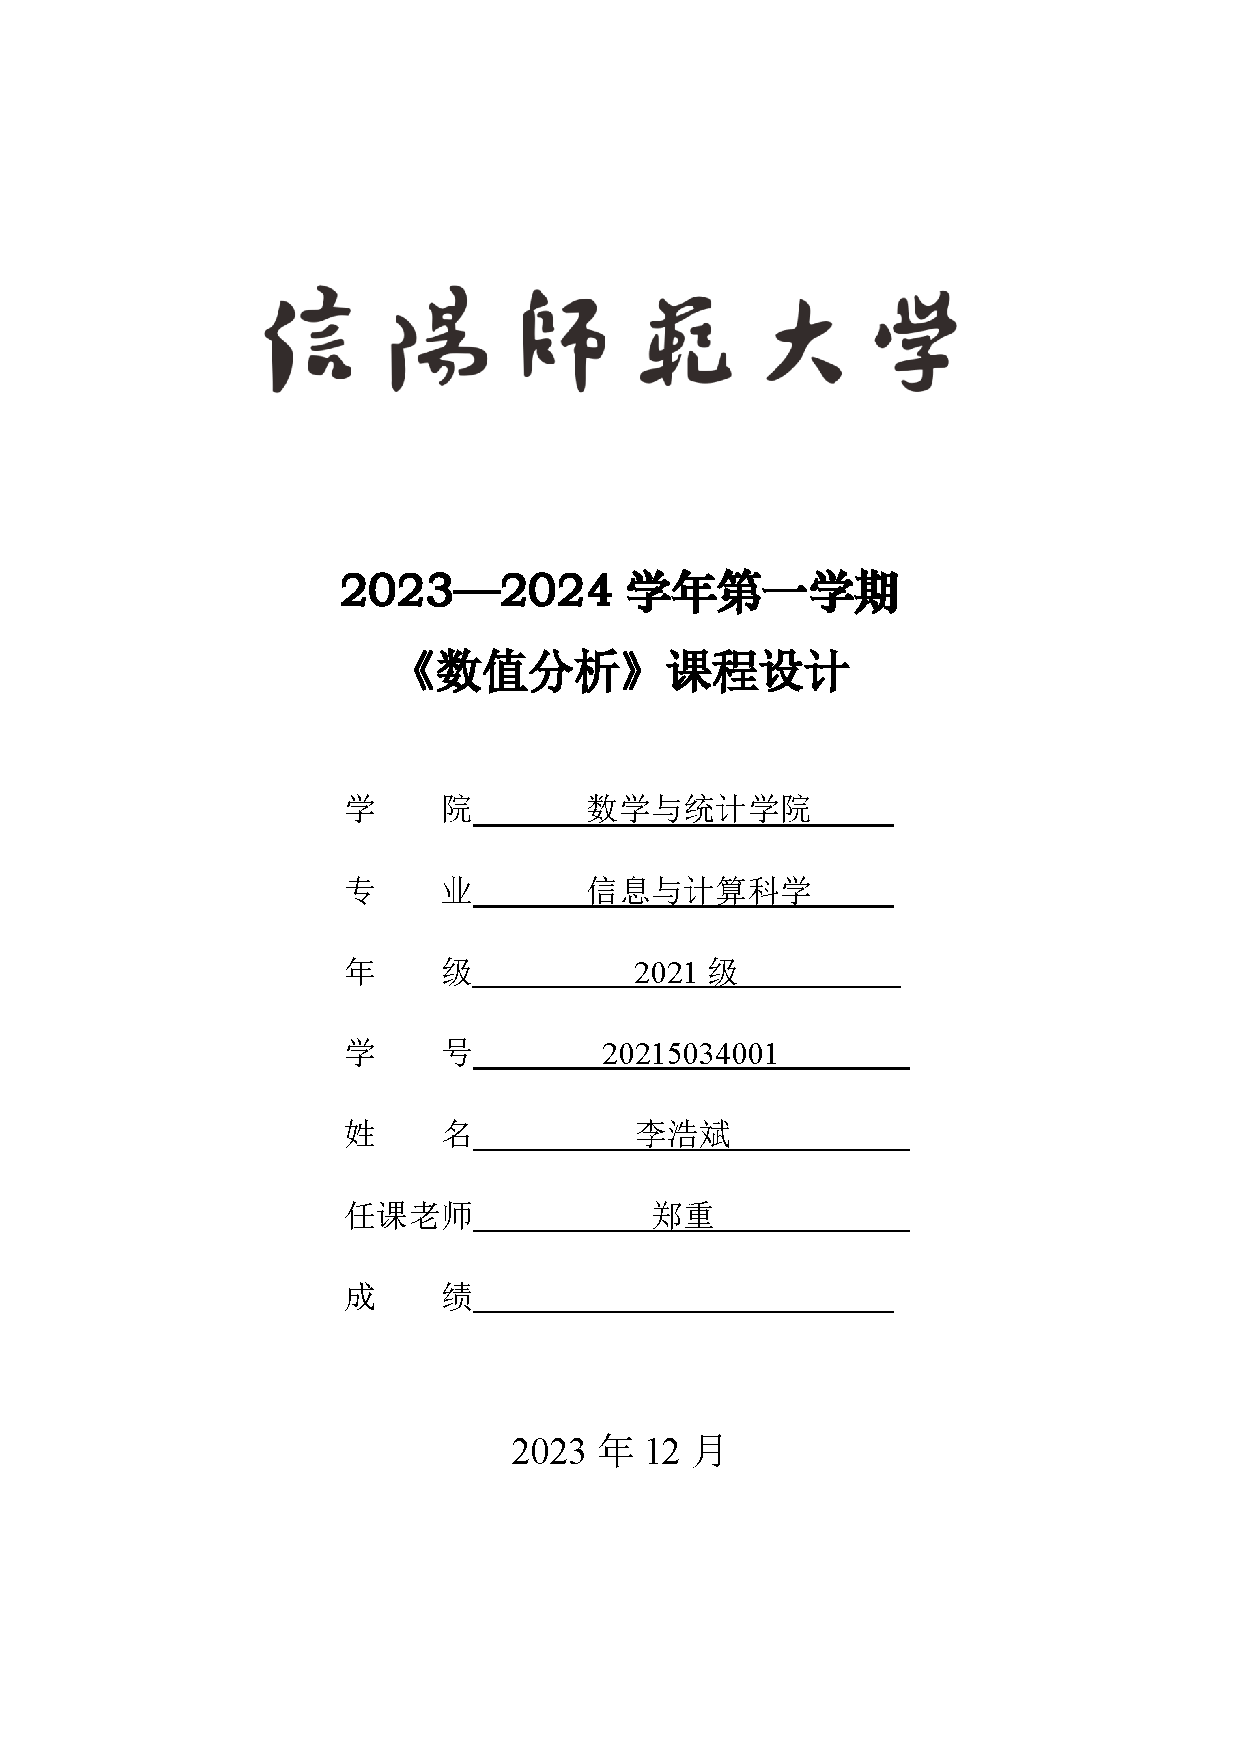
\includepdf{pageset/firstpage.pdf}
	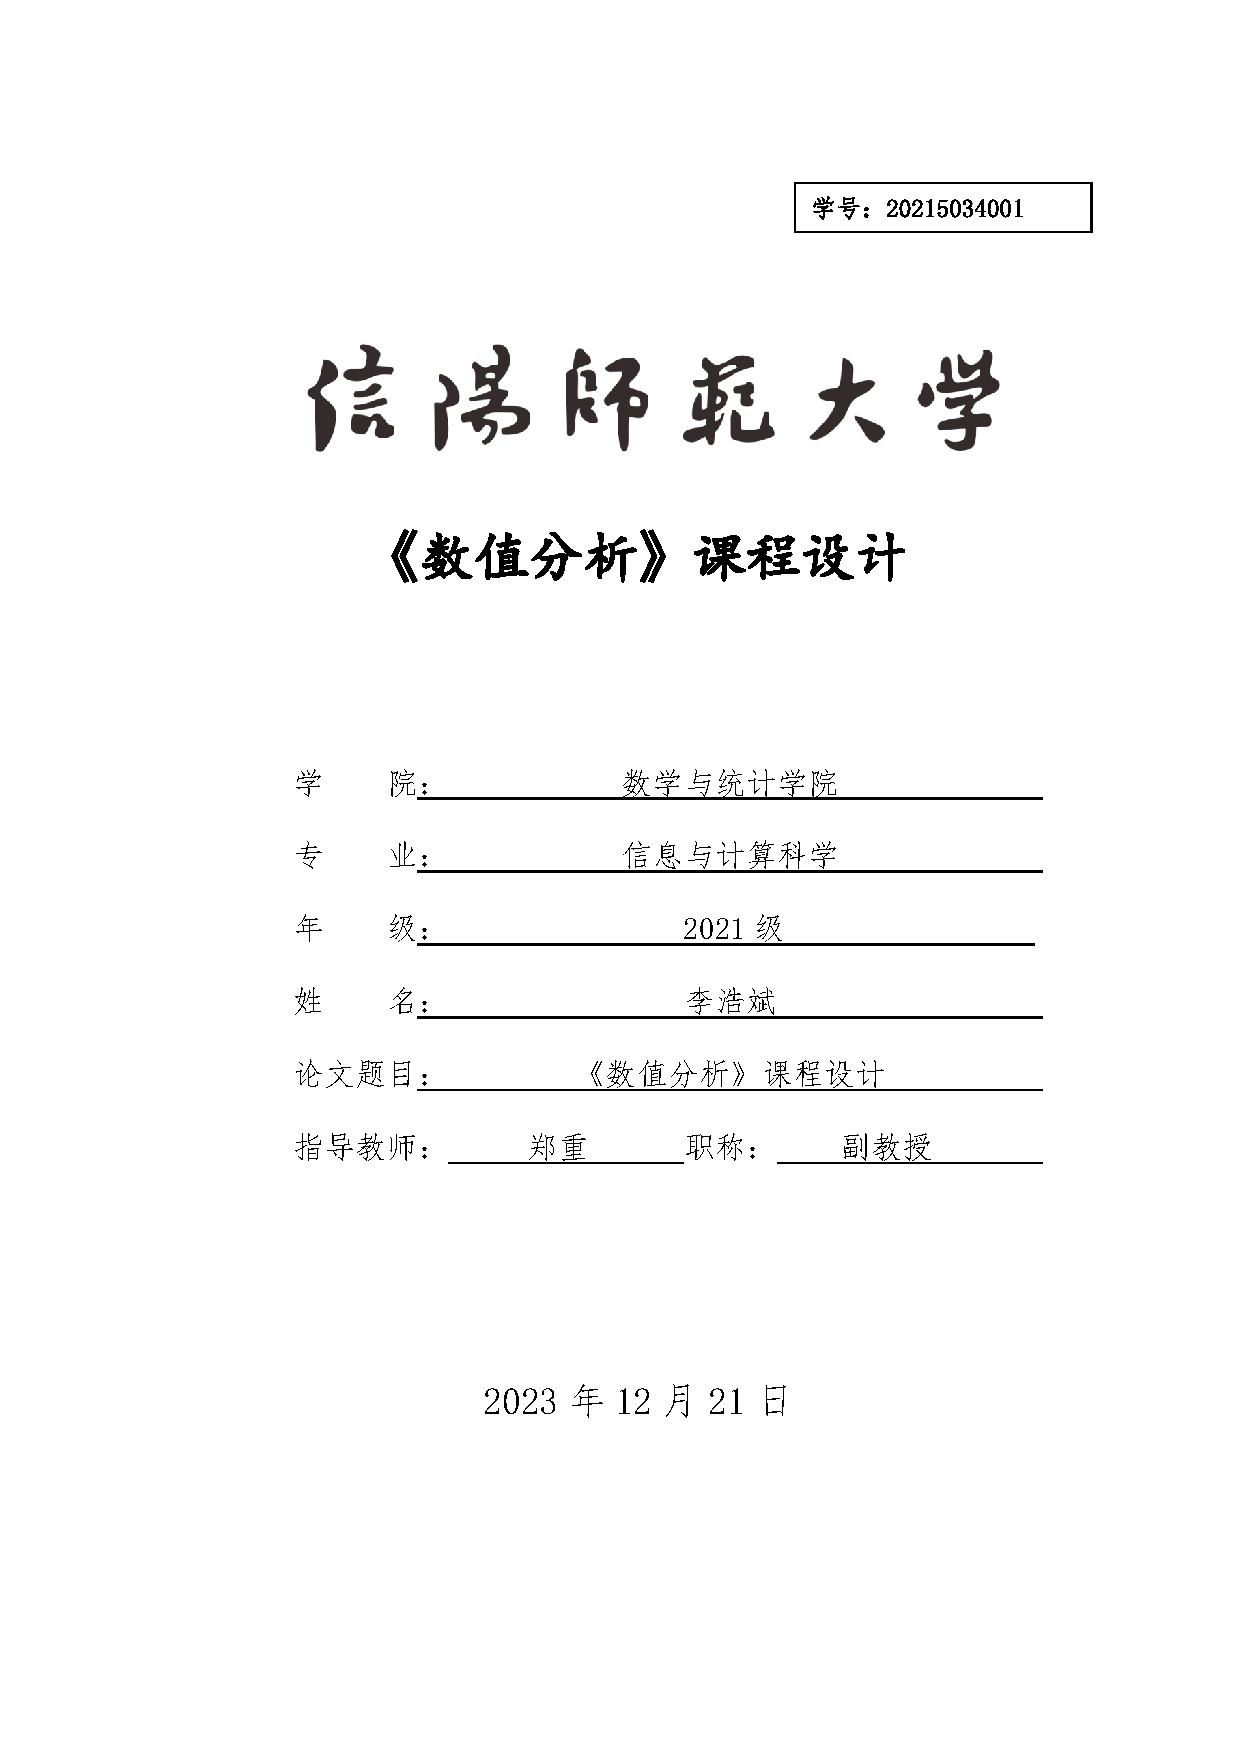
\includepdf{pageset/first.pdf}
	\newpage
	%\maketitle
	\tableofcontents
	\everymath{\displaystyle}
	\clearpage
	\ULCornerWallPaper{1}{pageset/coverpage.pdf}
	\section{第一周数值分析实验}
\subsection{第一节:级数求和与二元函数绘图}
\begin{ex}
编程求$\sum_{n=1}^{12}{n!}$的值.
\end{ex}
\lstinputlisting[language=matlab]{day1/work1q1.m}
\qa 522956313
\begin{ex}
绘制二元函数图像.
$$
f(x,y)=x^4-2x^2y+x^2-2xy+2y^2+\frac{9}{2}x-4y+4\,\,\,\,\left( -2\le x\le 3,-1\le y\le 7 \right) 
$$
\end{ex}
\lstinputlisting[language=matlab]{day1/work1q2.m}
\qa 
\begin{figure}[H]
	\centering
	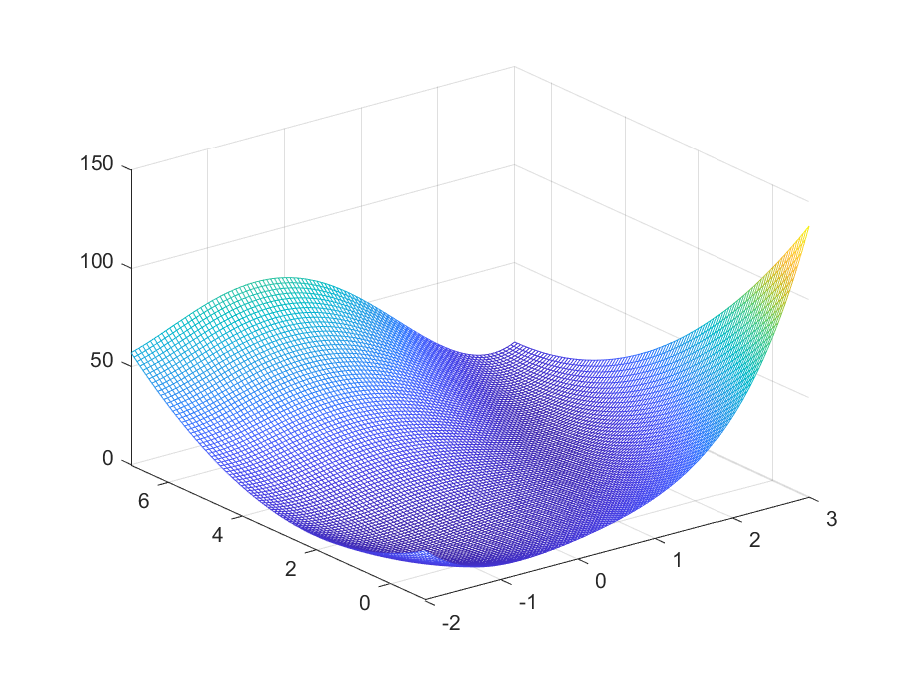
\includegraphics[width = 0.6\linewidth]{day1/q2.eps}
	\caption{运行结果}
\end{figure}
\subsection{第二节:积分递推公式}
\begin{ex}
	计算$I_n=e^{-1}\int_0^1{x^ne^xdx},(n=0,1,2,\cdots)$并估计误差
	
	方法1:利用递推公式 (A)
	$$
	\left( A \right) \text{ }\left\{ \begin{array}{l}
		I_n=1-nI_{n-1},\text{ }n=1,2,\cdots ,20\\
		I_0=1-e^{-1}\approx 0.6321.\\
	\end{array} \right. 
	$$
	
	方法2:利用递推公式 (B)
	$$
	\left( B \right) \left\{ \begin{array}{l}
		\widetilde{I_{20}}=?;\\
		\widetilde{I}_{n-1}=\frac{1}{n}\left( 1-\widetilde{I_n} \right) ,\text{ \,\,}n=19,\cdots ,9,8,\cdots 0.\\
	\end{array} \right. 
	$$
\end{ex}
\lstinputlisting[language=matlab]{day1/work1q3.m}
\qa 
% Table generated by Excel2LaTeX from sheet 'Sheet1'
\begin{table}[htbp]
	\centering
	\caption{运行结果}
	\resizebox{1\columnwidth}{!}{
	\begin{tabular}{c|cccccccccc}
		n     & 1     & 2     & 3     & 4     & 5     & 6     & 7     & 8     & 9     & 10 \\
		IA    & 0.3679 & 0.2642 & 0.2074 & 0.1704 & 0.148 & 0.112 & 0.216 & -0.728 & 7.552 & -74.52 \\
		EA    & 5.00E-05 & 5.00E-05 & 0.0001 & 0.0003 & 0.0012 & 0.006 & 0.036 & 0.252 & 2.016 & 18.144 \\
		n     & 11    & 12    & 13    & 14    & 15    & 16    & 17    & 18    & 19    & 20 \\
		IA    & 820.72 & -9847.64 & 128020.3 & -1792283 & 26884253 & -4.3E+08 & 7.31E+09 & -1.3E+11 & 2.5E+12 & -5E+13 \\
		EA    & 181.44 & 1995.84 & 23950.08 & 311351 & 4358915 & 65383718 & 1.05E+09 & 1.78E+10 & 3.2E+11 & 6.08E+12 \\
		\hline
		n     & 1     & 2     & 3     & 4     & 5     & 6     & 7     & 8     & 9     & 10 \\
		IB    & 0.367879 & 0.264241 & 0.207277 & 0.170893 & 0.145533 & 0.126802 & 0.112384 & 0.100932 & 0.091612 & 0.083877 \\
		EB    & 2.06E-20 & 4.11E-20 & 1.23E-19 & 4.93E-19 & 2.47E-18 & 1.48E-17 & 1.04E-16 & 8.29E-16 & 7.46E-15 & 7.46E-14 \\
		n     & 11    & 12    & 13    & 14    & 15    & 16    & 17    & 18    & 19    & 20 \\
		IB    & 0.077352 & 0.071773 & 0.066948 & 0.062732 & 0.059018 & 0.05572 & 0.052768 & 0.05018 & 0.04658 & 0.0684 \\
		EB    & 8.20E-13 & 9.84E-12 & 1.28E-10 & 1.79E-09 & 2.69E-08 & 4.30E-07 & 7.31E-06 & 0.000132 & 0.0025 & 0.05 \\
	\end{tabular}%
	}
	\label{tab:addlabel1}%
\end{table}%
\begin{ex}
	计算$I_n=\int_0^1{\frac{x^n}{x+5}dx},(n=0,1,2,\cdots 20)$并估计误差.
\end{ex}
\lstinputlisting[language=matlab]{day1/work1q4.m}
\qa 
% Table generated by Excel2LaTeX from sheet 'Sheet1'
\begin{table}[H]
	\centering
	\caption{运行结果}
	\resizebox{1\columnwidth}{!}{
	\begin{tabular}{c|cccccccccc}
		n     & 1     & 2     & 3     & 4     & 5     & 6     & 7     & 8     & 9     & 10 \\
		IA    & 0.0885 & 0.0575 & 0.045833 & 0.020833 & 0.095833 & -0.3125 & 1.705357 & -8.40179 & 42.12004 & -210.5 \\
		EA    & 5.00E-06 & 2.50E-05 & 0.000125 & 0.000625 & 0.003125 & 0.015625 & 0.078125 & 0.390625 & 1.953125 & 9.765625 \\
		n     & 11    & 12    & 13    & 14    & 15    & 16    & 17    & 18    & 19    & 20 \\
		IA    & 1052.592 & -5262.88 & 26314.46 & -131572 & 657861.2 & -3289306 & 16446529 & -8.2E+07 & 4.11E+08 & -2.1E+09 \\
		EA    & 48.82813 & 244.1406 & 1220.703 & 6103.516 & 30517.58 & 152587.9 & 762939.5 & 3814697 & 19073486 & 95367432 \\
		\hline
		n     & 1     & 2     & 3     & 4     & 5     & 6     & 7     & 8     & 9     & 10 \\
		IB    & 0.088392 & 0.058039 & 0.043139 & 0.034306 & 0.028468 & 0.024325 & 0.021233 & 0.018837 & 0.016926 & 0.015368 \\
		EB    & 2.62E-18 & 1.31E-17 & 6.55E-17 & 3.28E-16 & 1.64E-15 & 8.19E-15 & 4.10E-14 & 2.05E-13 & 1.02E-12 & 5.12E-12 \\
		n     & 11    & 12    & 13    & 14    & 15    & 16    & 17    & 18    & 19    & 20 \\
		IB    & 0.014071 & 0.012977 & 0.01204 & 0.011229 & 0.010521 & 0.009896 & 0.009342 & 0.008846 & 0.008402 & 0.00799 \\
		EB    & 2.56E-11 & 1.28E-10 & 6.40E-10 & 3.20E-09 & 1.60E-08 & 8.00E-08 & 4.00E-07 & 2.00E-06 & 1.00E-05 & 5.00E-05 \\
	\end{tabular}%
	}
	\label{tab:addlabel2}%
\end{table}%

	\section{第二周数值分析实验}
\subsection{第一节:插值function}
\subsubsection{直接法}
\lstinputlisting[language=matlab]{day2/Vslove.m}
\subsubsection{Lagrange法}
\lstinputlisting[language=matlab]{day2/lagrangeslove.m}
\subsection{第二节:计算实例}
\begin{ex}
	给出插值点
	$$x = (0.25, 0.3, 0.39, 0.45, 0.53, 0.66, 0.72)^T,$$  
	$$y = (0.5, 0.5477, 0.6245, 0.6708, 0.7280, 1.0254, 0.9521)^T .$$ 
	时的两种方法插值多项式表达式及对应的函数图像, 并与MATLAB拟合工具箱(cftool)进行比较.
\end{ex}
\subsubsection{直接法计算}
\lstinputlisting[language=matlab]{day2/mainvslove.m}
\subsubsection{Lagrange法计算}
\lstinputlisting[language=matlab]{day2/mainlagrange.m}
\subsubsection{结果}
\begin{figure}[H]
	\centering
	\subfloat[直接法图像]{\includegraphics[width = 0.5\linewidth]{day2/fig1.eps}}
	\hfill
	\subfloat[Lagrange法图像]{\includegraphics[width = 0.5\linewidth]{day2/fig2.eps}}
	\caption{运行结果}
	\label{fig:cj12}
\end{figure}

	\section{第三周数值分析实验}
\subsection{Newton法均差表function}
\lstinputlisting[language=matlab]{day3/newtonmatrix.m}
\subsection{\texttt{page32ex4}实例}
\lstinputlisting[language=matlab]{day3/main.m}
\subsubsection{结果}
\begin{figure}[H]
	\centering
	\includegraphics[width = 0.6\linewidth]{day3/newton.eps}
	\caption{Newton法结果}
\end{figure}


	\section{第四周数值分析实验}
\begin{ex}
	自行选择节点,构造插值多项式,并估计$\sqrt{2},\sqrt{2.2},\sqrt{2.5}$的值.
	\begin{itemize}
		\item 不得使用牛顿切线法;
		\item 不得涉及无理数运算;
		\item 有效数字位数不少于$5$位.
	\end{itemize}
\end{ex}
\subsection{三点三次Hermite插值}
\lstinputlisting[language=matlab]{day4/work4h33.m}
\qa [1.4142, 1.4832, 1.5811]
\subsection{两点三次Hermite插值}
\lstinputlisting[language=matlab]{day4/work4h23.m}
\qa [1.4142, 1.4833, 1.5811]
\begin{figure}[H]
	\centering
	\subfloat[三点三次Hermite插值]{\includegraphics[width = 0.5\linewidth]{day4/h33.eps}}
	\hfill
	\subfloat[两点三次Hermite插值]{\includegraphics[width = 0.5\linewidth]{day4/h23.eps}}
	\caption{运行结果}
	\label{fig:day4}
\end{figure}


	\section{第六周数值分析实验}
\subsection{Bernstein多项式}
\begin{definition}
	设$f:[0,1]\to\mathbb{R}$,称
	$$
	B_n(f;x)=\sum_{i=0}^{n}f\left(\frac{i}{n}\right)B_i^n(x),x\in[0,1]
	$$
	为$f$的$n$次Bernstein多项式,其中$B_i^n(x)=\binom{n}{i}x^i(1-x)^{n-i}$.
\end{definition}
\lstinputlisting[language=matlab]{day5/bernstein_n.m}
\begin{ex}
	当$f(x)=\cos 2\pi x$时,分别给出$n=3, 5, 7, 9, 10$时的$B_n(f,x)$表达式,并绘制$f(x)$与$B_n(f,x)$的图像.
\end{ex}
\lstinputlisting[language=matlab]{day5/main.m}
\begin{figure}[H]
	\centering
	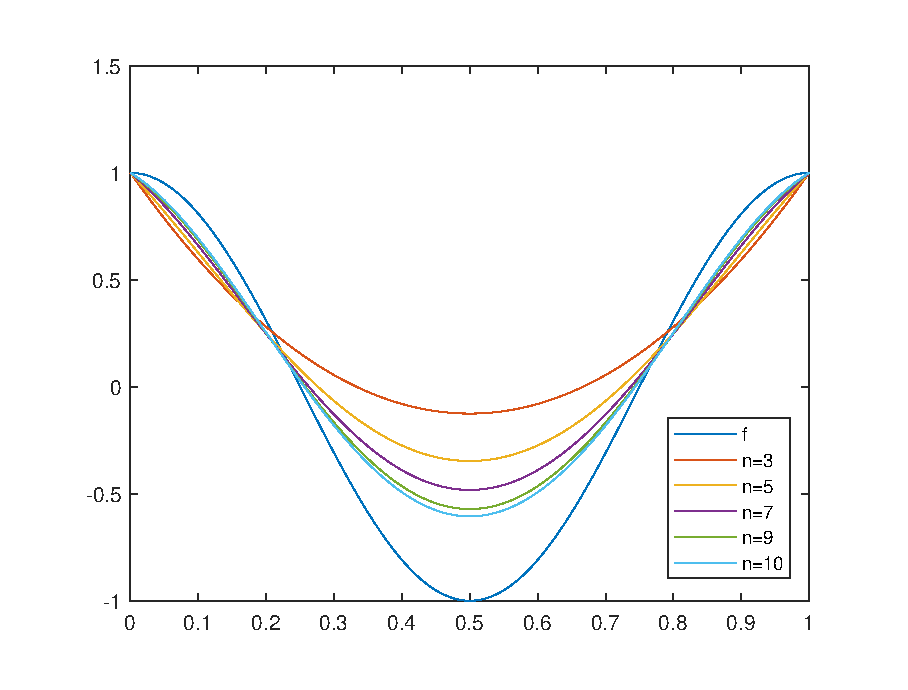
\includegraphics[width = 0.6\linewidth]{day5/fig.eps}
	\caption{Bernstein多项式图像}
\end{figure}
	\section{第七周数值分析实验}
\subsection{Gram-Schmidt正交化}
\begin{ex}
	编程实现幂函数使用施密特正交化方法生成正交多项式
	
	施密特正交化:只要给定$[a,b]$上的权函数$\rho \left( x \right),$由$\{1,x,\cdots x^n,\cdots \}$利用逐个正交化立得正交多项式序列.
	$$
	\begin{aligned}
		& \varphi_0(x)=1, \\
		& \varphi_1(x)=x, \\
		& \varphi_2(x)=x^2-\frac{\left(x^2, \varphi_0\right)}{\left(\varphi_0, \varphi_0\right)} \varphi_0(x)-\frac{\left(x^2, \varphi_1\right)}{\left(\varphi_1, \varphi_1\right)} \varphi_1(x), \\
		& \varphi_n(x)=x^n-\sum_{j=0}^{n-1} \frac{\left(x^n, \varphi_j\right)}{\left(\varphi_j, \varphi_j\right)} \varphi_j(x), \quad n=3,4, \cdots .
	\end{aligned}
	$$
	或利用递推公式:
	$$
	\varphi_{n+1}(x)=\left(x-\alpha_n\right) \varphi_n(x)-\beta_n \varphi_{n-1}(x), n=0,1, \cdots
	$$
	其中
	$$
	\begin{aligned}
		& \varphi_0(x)=1, \varphi_{-1}(x)=0, \\
		& \alpha_n=\frac{\left(x \varphi_n(x), \varphi_n(x)\right)}{\left(\varphi_n(x), \varphi_n(x)\right)}, \beta_n=\frac{\left(\varphi_n(x), \varphi_n(x)\right)}{\left(\varphi_{n-1}(x), \varphi_{n-1}(x)\right)}, \\
		& \text { 这里 }\left(x \varphi_n(x), \varphi_n(x)\right)=\int_a^b x \varphi_n^2(x) \rho(x) d x .
	\end{aligned}
	$$
\end{ex}
\lstinputlisting[language=matlab]{day6/Schmidt1.m}
\subsection{Schmidt正交化-Legendre多项式}
\lstinputlisting[language=mathematica]{day6/schmidtlegendre.wl}
\qa (Mathematica)
\begin{figure}[H]
	\centering
	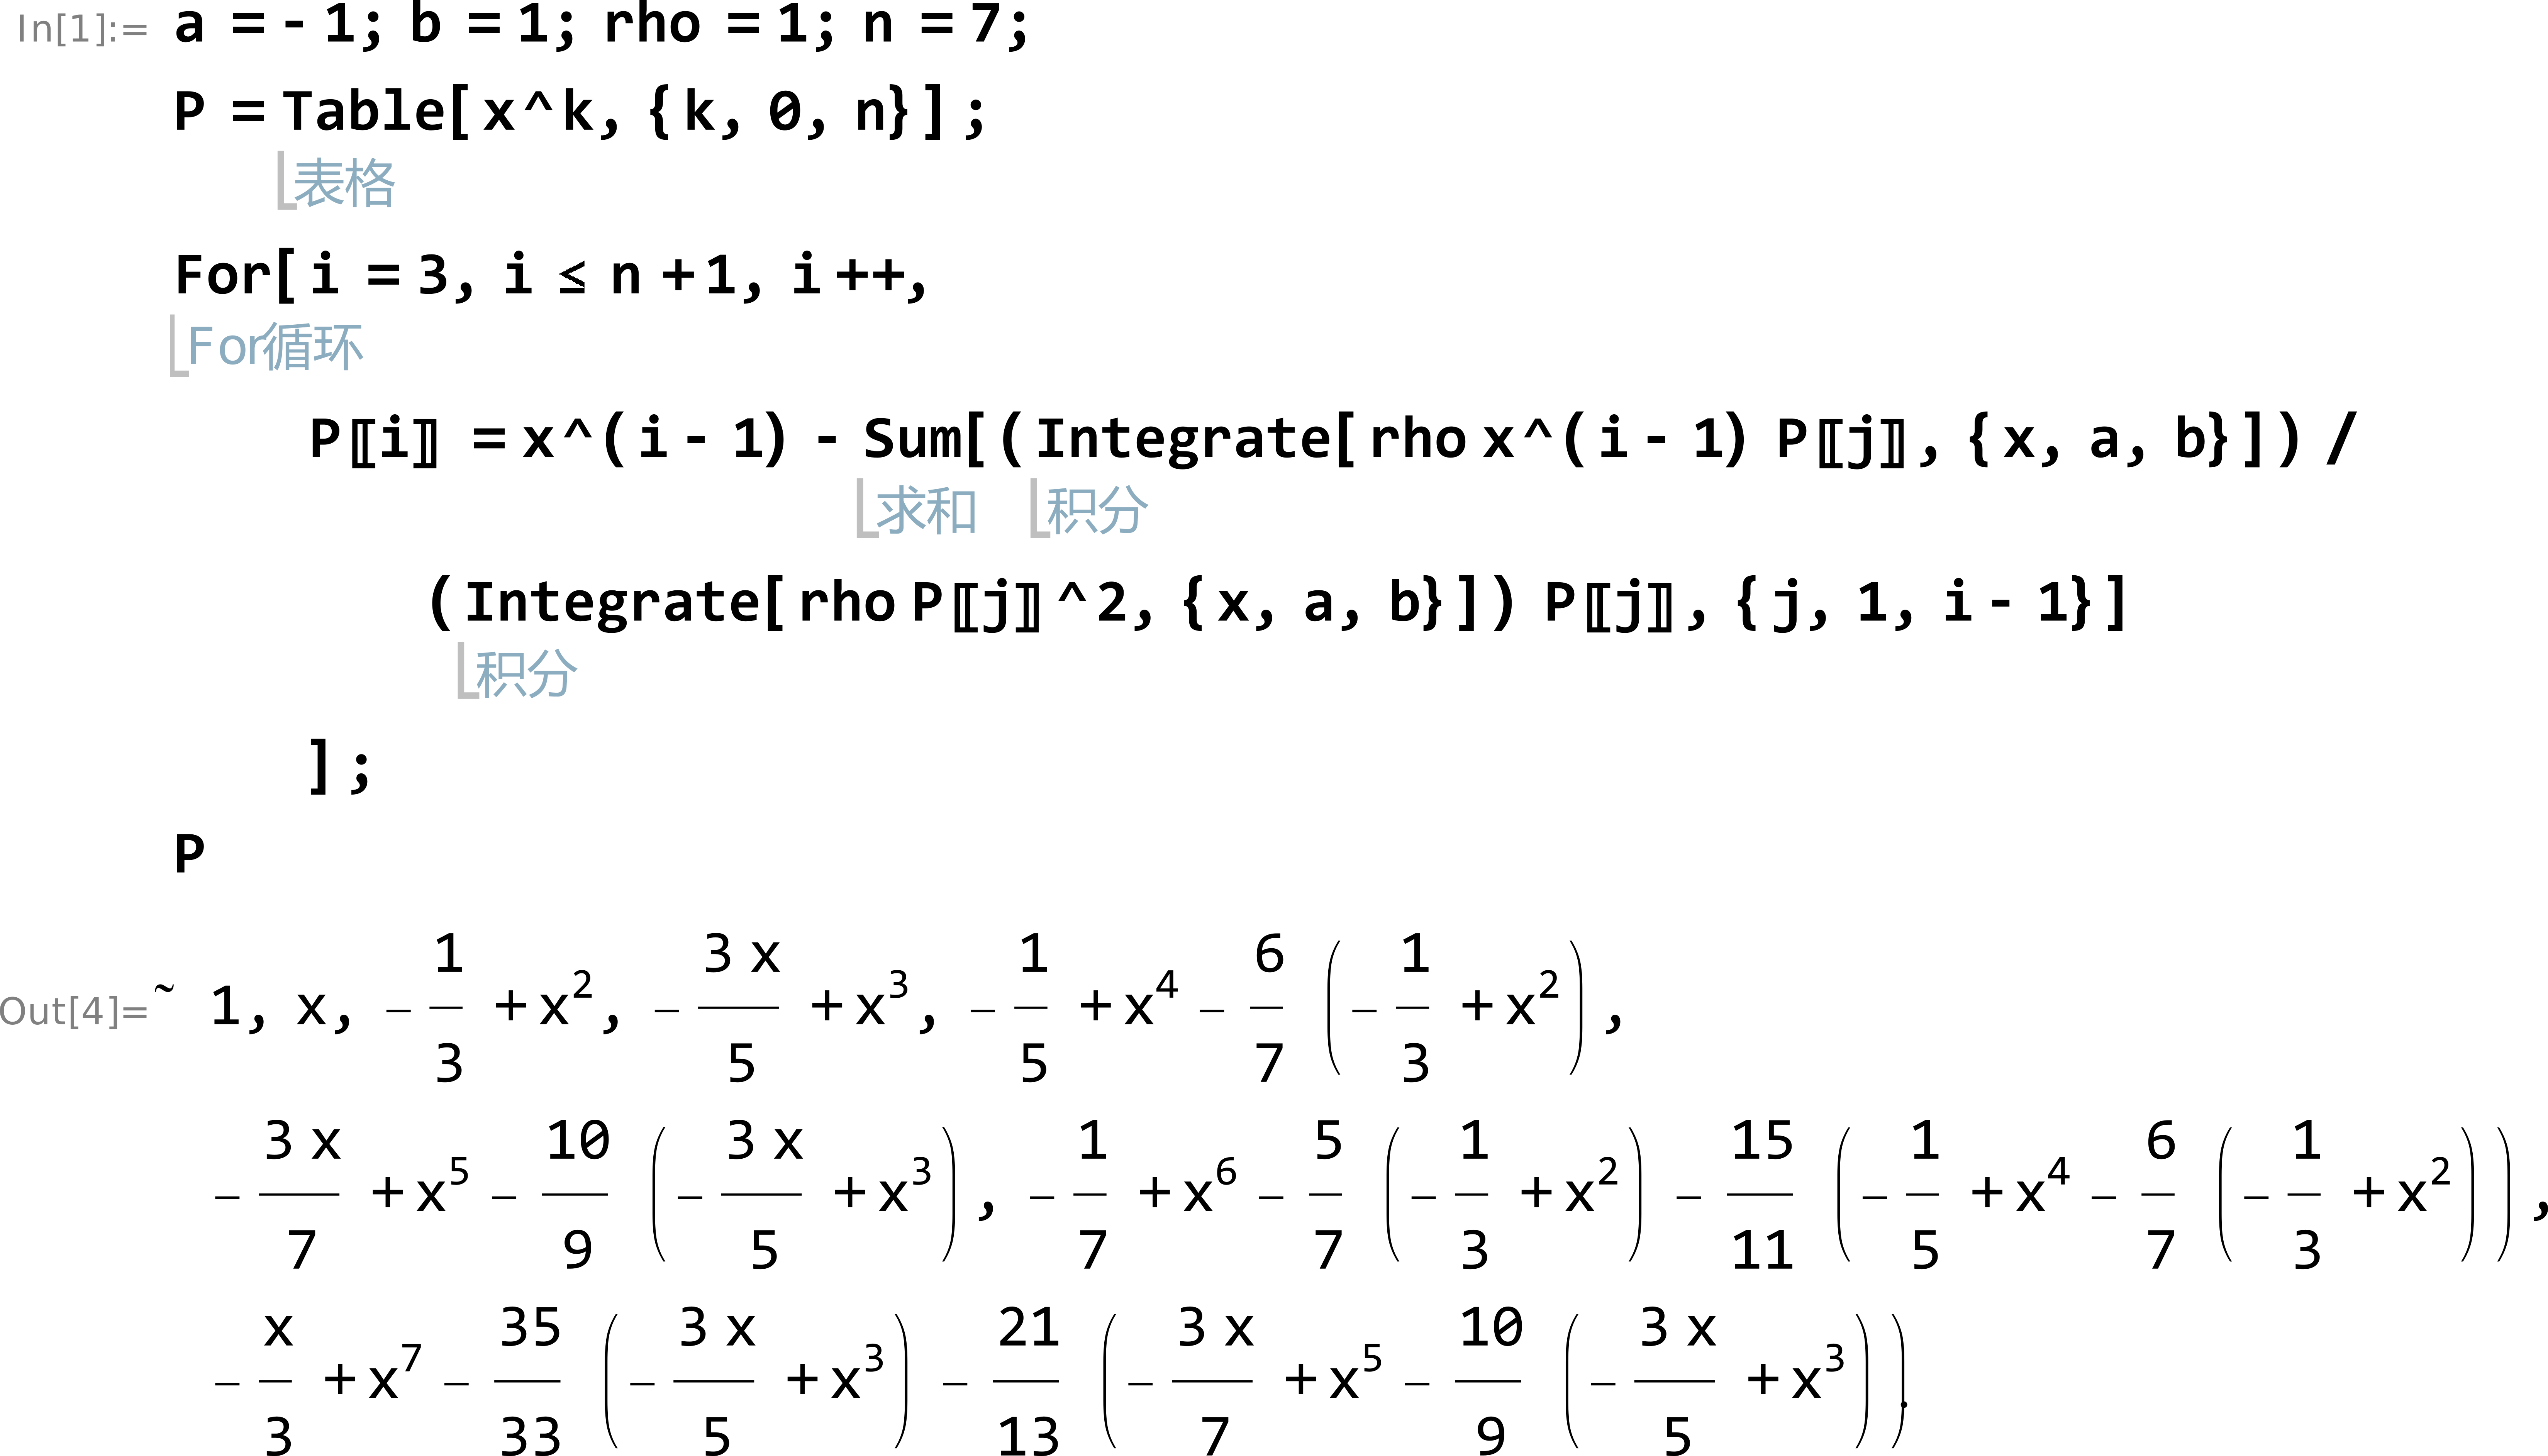
\includegraphics[width = 1\linewidth]{day6/fig1.png}
	\caption{Legendre}
\end{figure}
\subsection{Schmidt正交化-Chebyshev多项式}
\lstinputlisting[language=mathematica]{day6/schmidtchebyshev.wl}
\qa (Mathematica)
\begin{figure}[H]
	\centering
	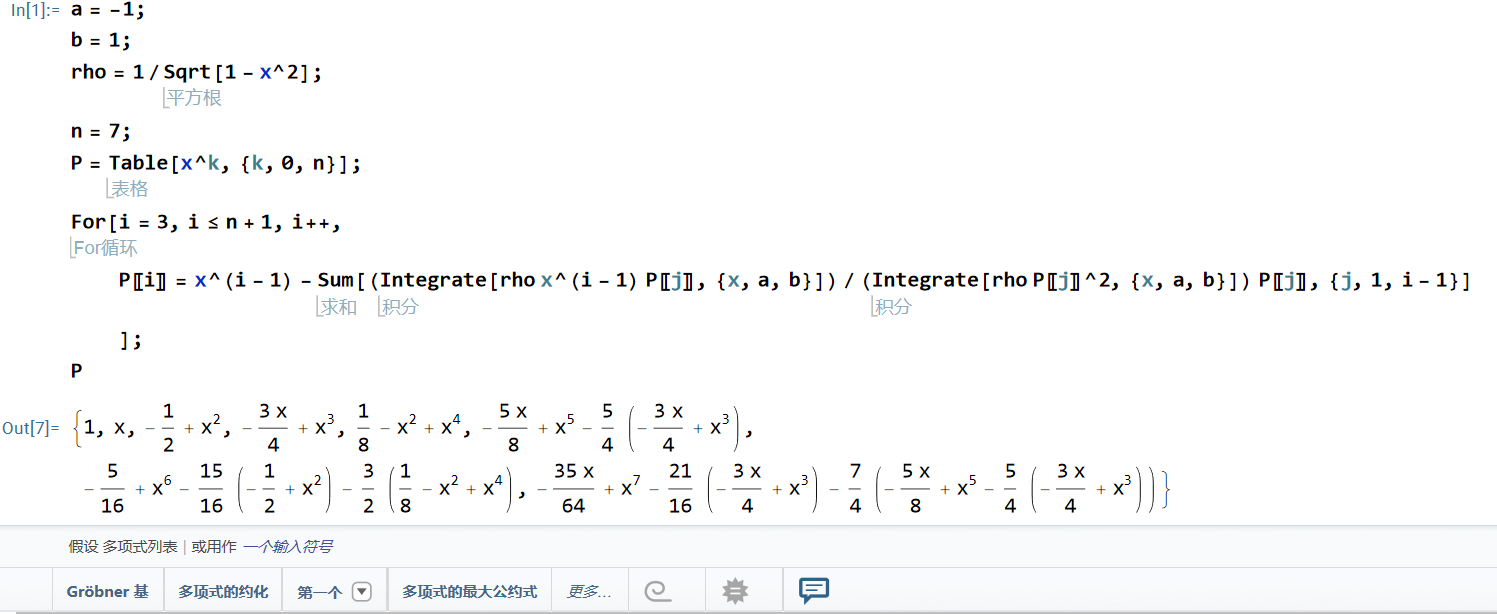
\includegraphics[width = 1\linewidth]{day6/fig2.png}
	\caption{Chebyshev}
\end{figure}
\subsection{递推法-Legendre多项式}
\lstinputlisting[language=matlab]{day6/legendremap.m}

	\section{第八周数值分析实验}
\subsection{第一题}
\begin{ex}
	设 $f(x)=\frac{1}{1+x^2}$, 在 $[-5,5]$ 上分别利用 $T_{11}(x), T_{15}(x), T_{21}(x)$ 的零点作为插值点,构造 $10$ 次, $14$ 次, $20 $次插值多项式 $L_{10}(x), L_{14}(x), L_{20}(x)$, 并作图表示; 此外, 作出误差曲线 $f(x)-L_{10}(x), f(x)-L_{14}(x), f(x)-L_{20}(x)$.
\end{ex}
\lstinputlisting[language=matlab]{day7/chebyshev.m}
%\begin{figure}[H]
%	\centering
%	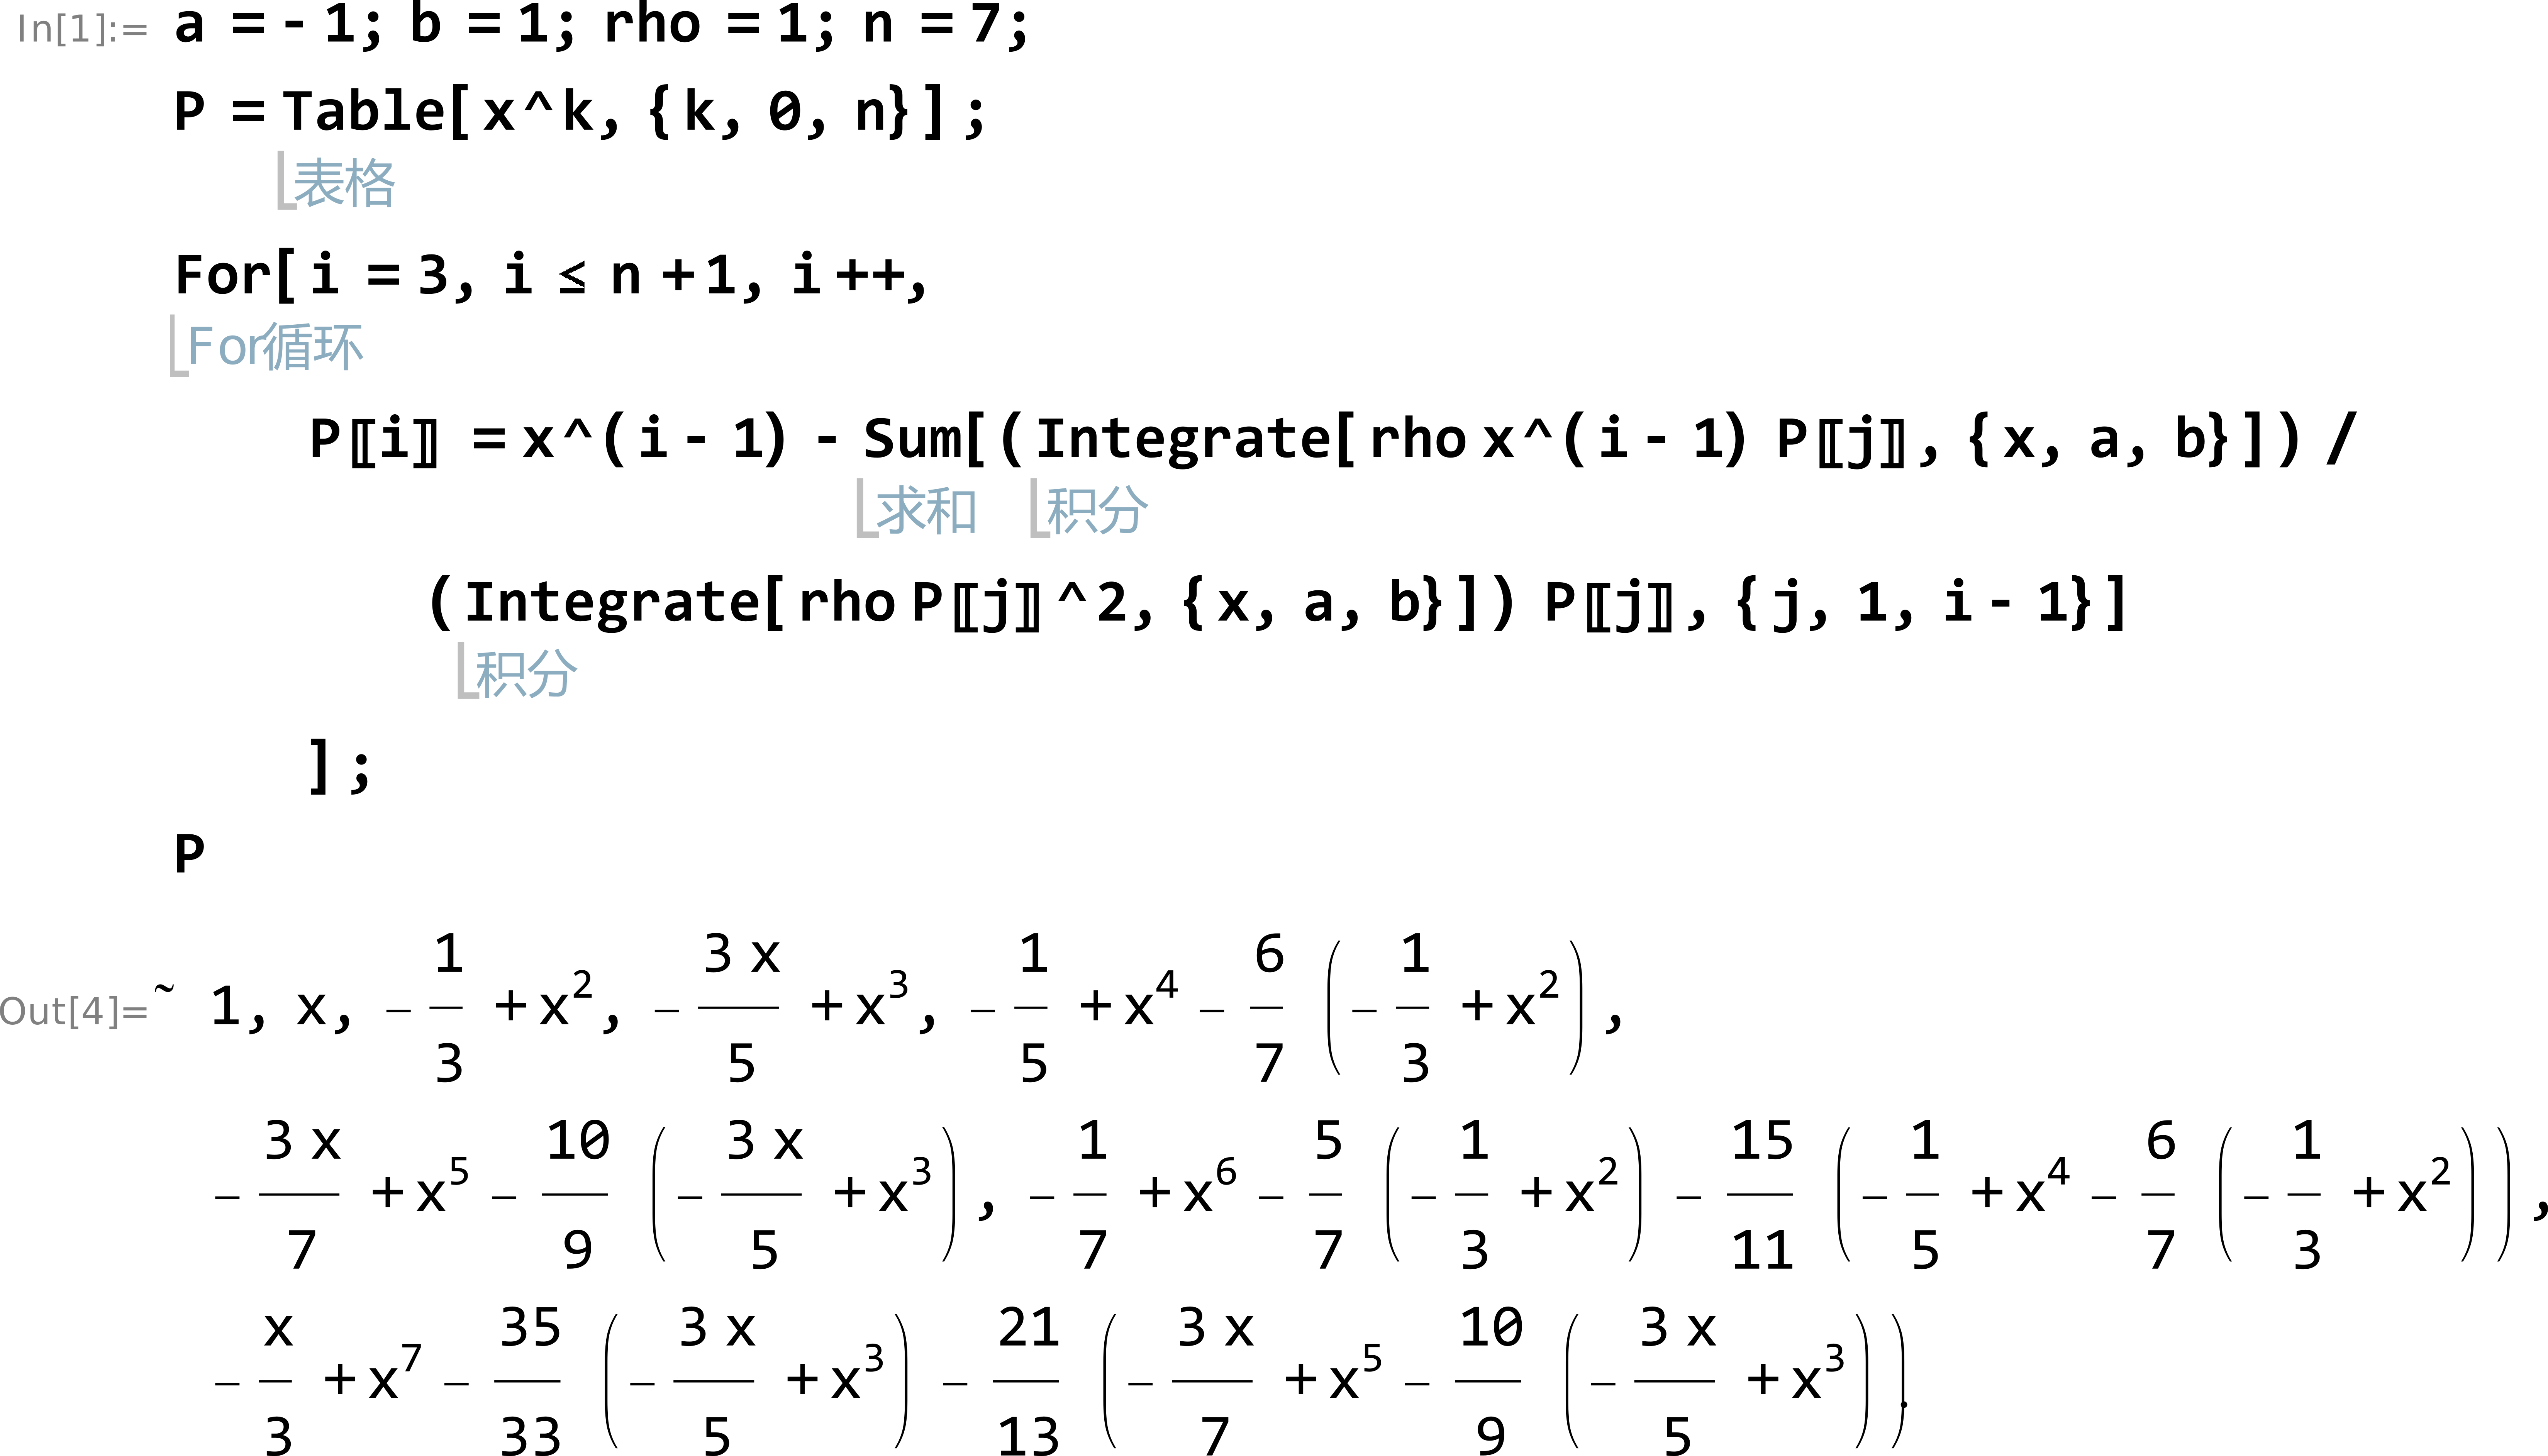
\includegraphics[width = 1\linewidth]{day6/fig1.png}
%	\caption{图示}
%\end{figure}
\begin{figure}[H]
	\centering
	\subfloat[Lagrange插值多项式图像]{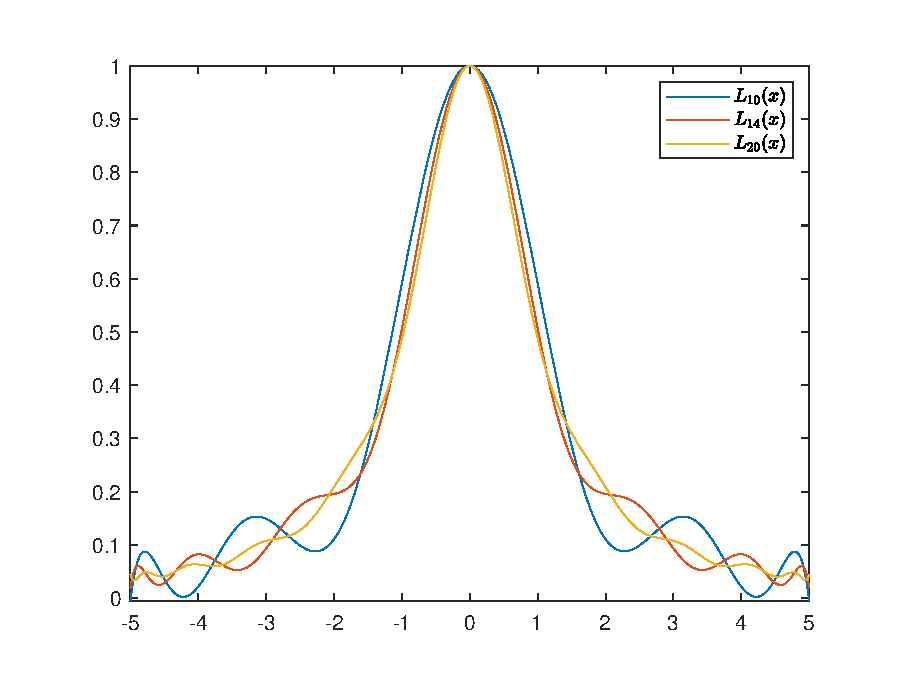
\includegraphics[width = 0.5\linewidth]{day7/q1fig1.eps}}
	\hfill
	\subfloat[误差曲线$f(x)-L_n(x)$]{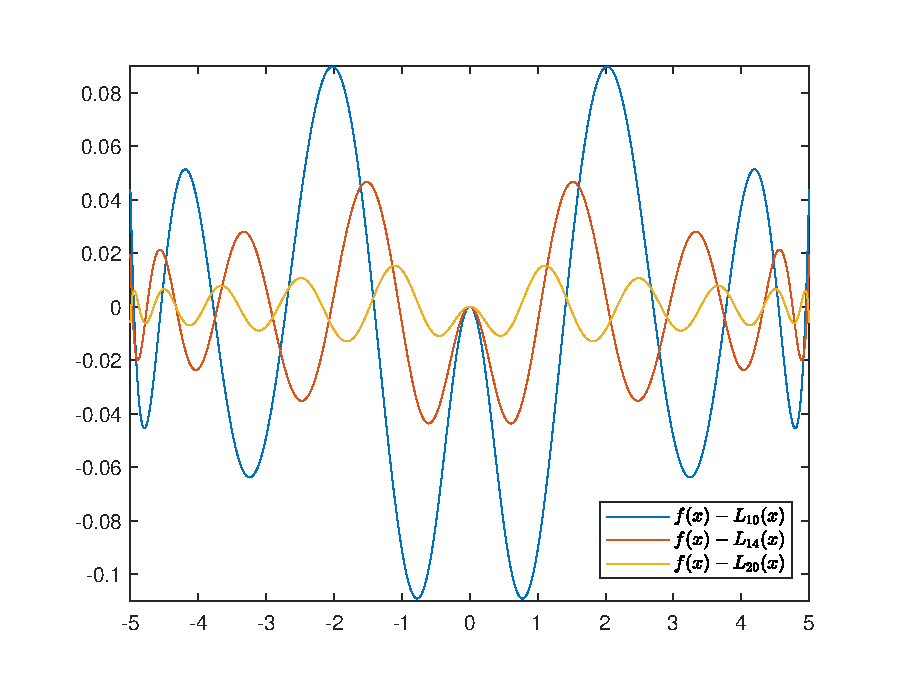
\includegraphics[width = 0.5\linewidth]{day7/q1fig2.eps}}
	\caption{结果图示}
\end{figure}
\subsection{第二题}
\begin{ex}
	设 $f(x)=2 x^4-3 x^3+2 x-1$, 绘制 $[0,1]$ 上的三次最佳一致逼近多项式 $P_3(x)$,二次最佳平方逼近多项式 $S_2(x)$, 伯恩斯坦多项式 $B_1(f, x), B_2(f, x), B_3(f, x)$.
\end{ex}
\lstinputlisting[language=matlab]{day7/q2.m}
	\section{第九周数值分析实验}
\subsection{正交函数族最佳平方逼近}
\begin{ex}
	设 $f(x)=\frac{1}{1+25 x^2}, x \in[-1,1]$, 利用勒让德正交多项式族, 分别构造 $3$ 次, $6$ 次, $10$ 次最佳平方逼近多项式, 并绘图与 $f(x)$ 比较.
\end{ex}
\lstinputlisting[language=matlab]{w9/legendremap.m}
\lstinputlisting[language=matlab]{w9/work9q1.m}
\begin{figure}[H]
	\centering
	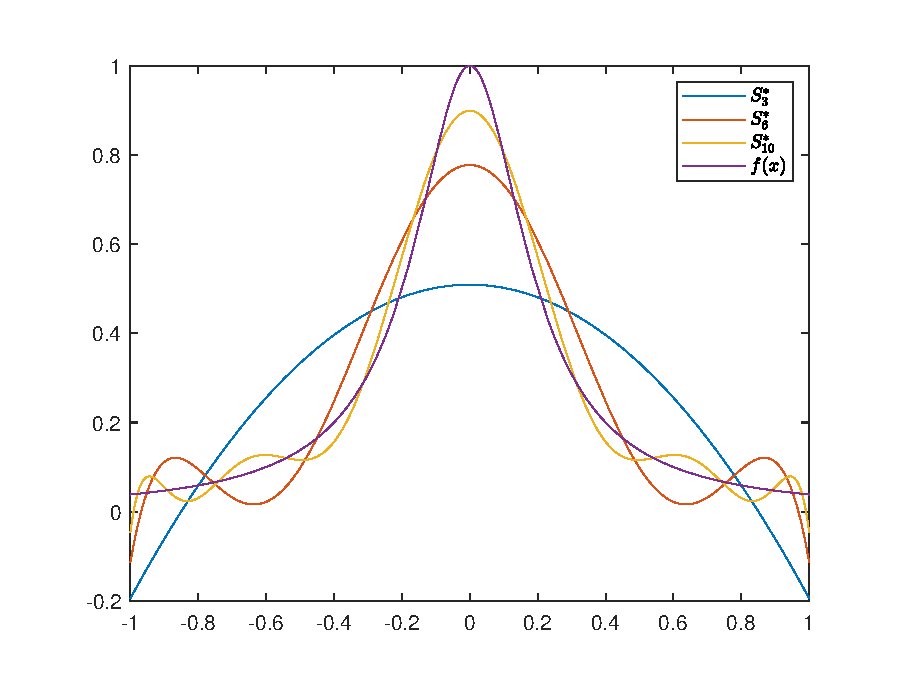
\includegraphics[width = 0.61\linewidth]{w9/figq1.eps}
	\caption{最佳平方逼近}
\end{figure}
\subsection{最小二乘拟合}
\begin{ex}
	实验数据如下
	
	\begin{tabular}{|c|c|c|c|c|c|c|c|c|c|c|c|c|}
		\hline$x_i$ & -1 & -0.8 & -0.6 & -0.4 & -0.3 & -0.1 & 0 & 0.2 & 0.4 & 0.6 & 0.8 & 1 \\
		\hline $y_i$ & 0 & 1.27 & 2.16 & 2.86 & 3.44 & 3.87 & 4.15 & 4.37 & 4.51 & 4.58 & 4.62 & 4.64 \\
		\hline
	\end{tabular}
	
	(1) 确定法方程组, 并求$ 2 $次及$ 3 $次拟合多项式函数 $s=s(x)$;
	
	(2) 与MATLAB拟合工具箱cftool对比.
\end{ex}
\lstinputlisting[language=matlab]{w9/work9q2.m}
\begin{figure}[H]
	\centering
	\subfloat[二次拟合多项式]{\includegraphics[width = 0.5\linewidth]{w9/figq21.eps}}
	\hfill
	\subfloat[三次拟合多项式]{\includegraphics[width = 0.5\linewidth]{w9/figq22.eps}}
	\hfill
	\subfloat[二次拟合多项式]{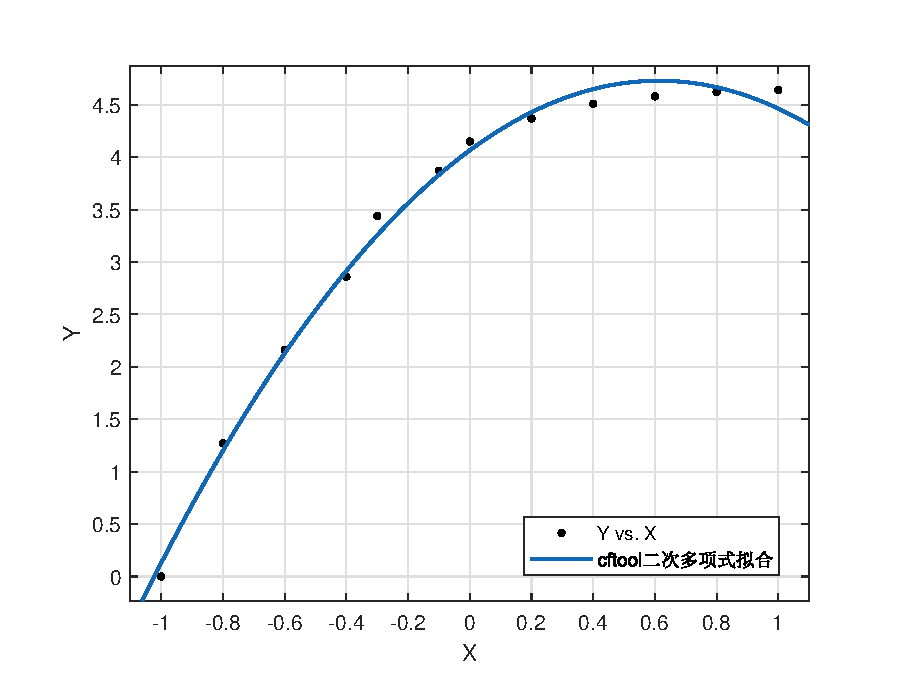
\includegraphics[width = 0.5\linewidth]{w9/figq2c1.eps}}
	\hfill
	\subfloat[三次拟合多项式]{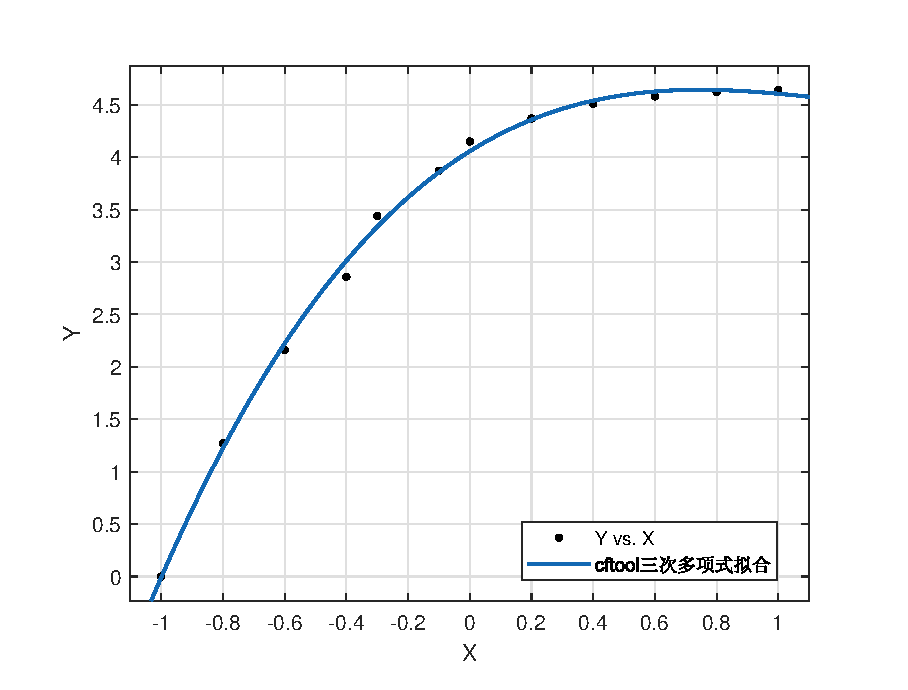
\includegraphics[width = 0.5\linewidth]{w9/figq2c2.eps}}
	\caption{最小二乘拟合}
\end{figure}

	\section{第十周数值分析中期练习}
\subsection{三次插值}
\begin{ex}
已知 $y=f(x)$ 的在部分节点上的函数值如下表所示:
\begin{table}[H]
	\centering
	\begin{tabular}{|c|c|c|c|c|}
		\hline$x_i$ & -2 & 0 & 1 & 2 \\
		\hline$f\left(x_i\right)$ & -7 & 1 & 2 & 9 \\
		\hline
	\end{tabular}
\end{table}
	试构造三次插值多项式, 并估计在 $x=1.3$ 处的值。
\end{ex}
\lstinputlisting[language=matlab]{w10/q1.m}
\qa $x^3+1$;
3.1970e+000
\subsection{最小二乘法}
\begin{ex}
	已知实验数据如下:
	\begin{table}[H]
		\centering
		\begin{tabular}{|c|c|c|c|c|c|c|}
			\hline$x_i$ & 10 & 11 & 12 & 13 & 14 & 15 \\
			\hline$f\left(x_i\right)$ & 20 & 23 & 25 & 27 & 26 & 28 \\
			\hline
		\end{tabular}
	\end{table}
	请列出用最小二乘法求线性及二次拟合函数的方程组。
\end{ex}
\lstinputlisting[language=matlab]{w10/q2.m}
\qa 
\begin{flalign*}
	\begin{split}
		y=\frac{51\,x}{35}+\frac{1863096274418193}{281474976710656}.
	\end{split}&
\end{flalign*}
\begin{flalign*}
	\begin{split}
		y=-\frac{683582086296581\,x^2}{2251799813685248}+\frac{5092686542910377\,x}{562949953421312}-\frac{5619446856466419}{140737488355328}.
	\end{split}&
\end{flalign*}
\begin{figure}[H]
	\centering
	\subfloat[一次拟合多项式]{\includegraphics[width = 0.5\linewidth]{w10/q21.eps}}
	\hfill
	\subfloat[二次拟合多项式]{\includegraphics[width = 0.5\linewidth]{w10/q22.eps}}
	\caption{最小二乘法}
\end{figure}
%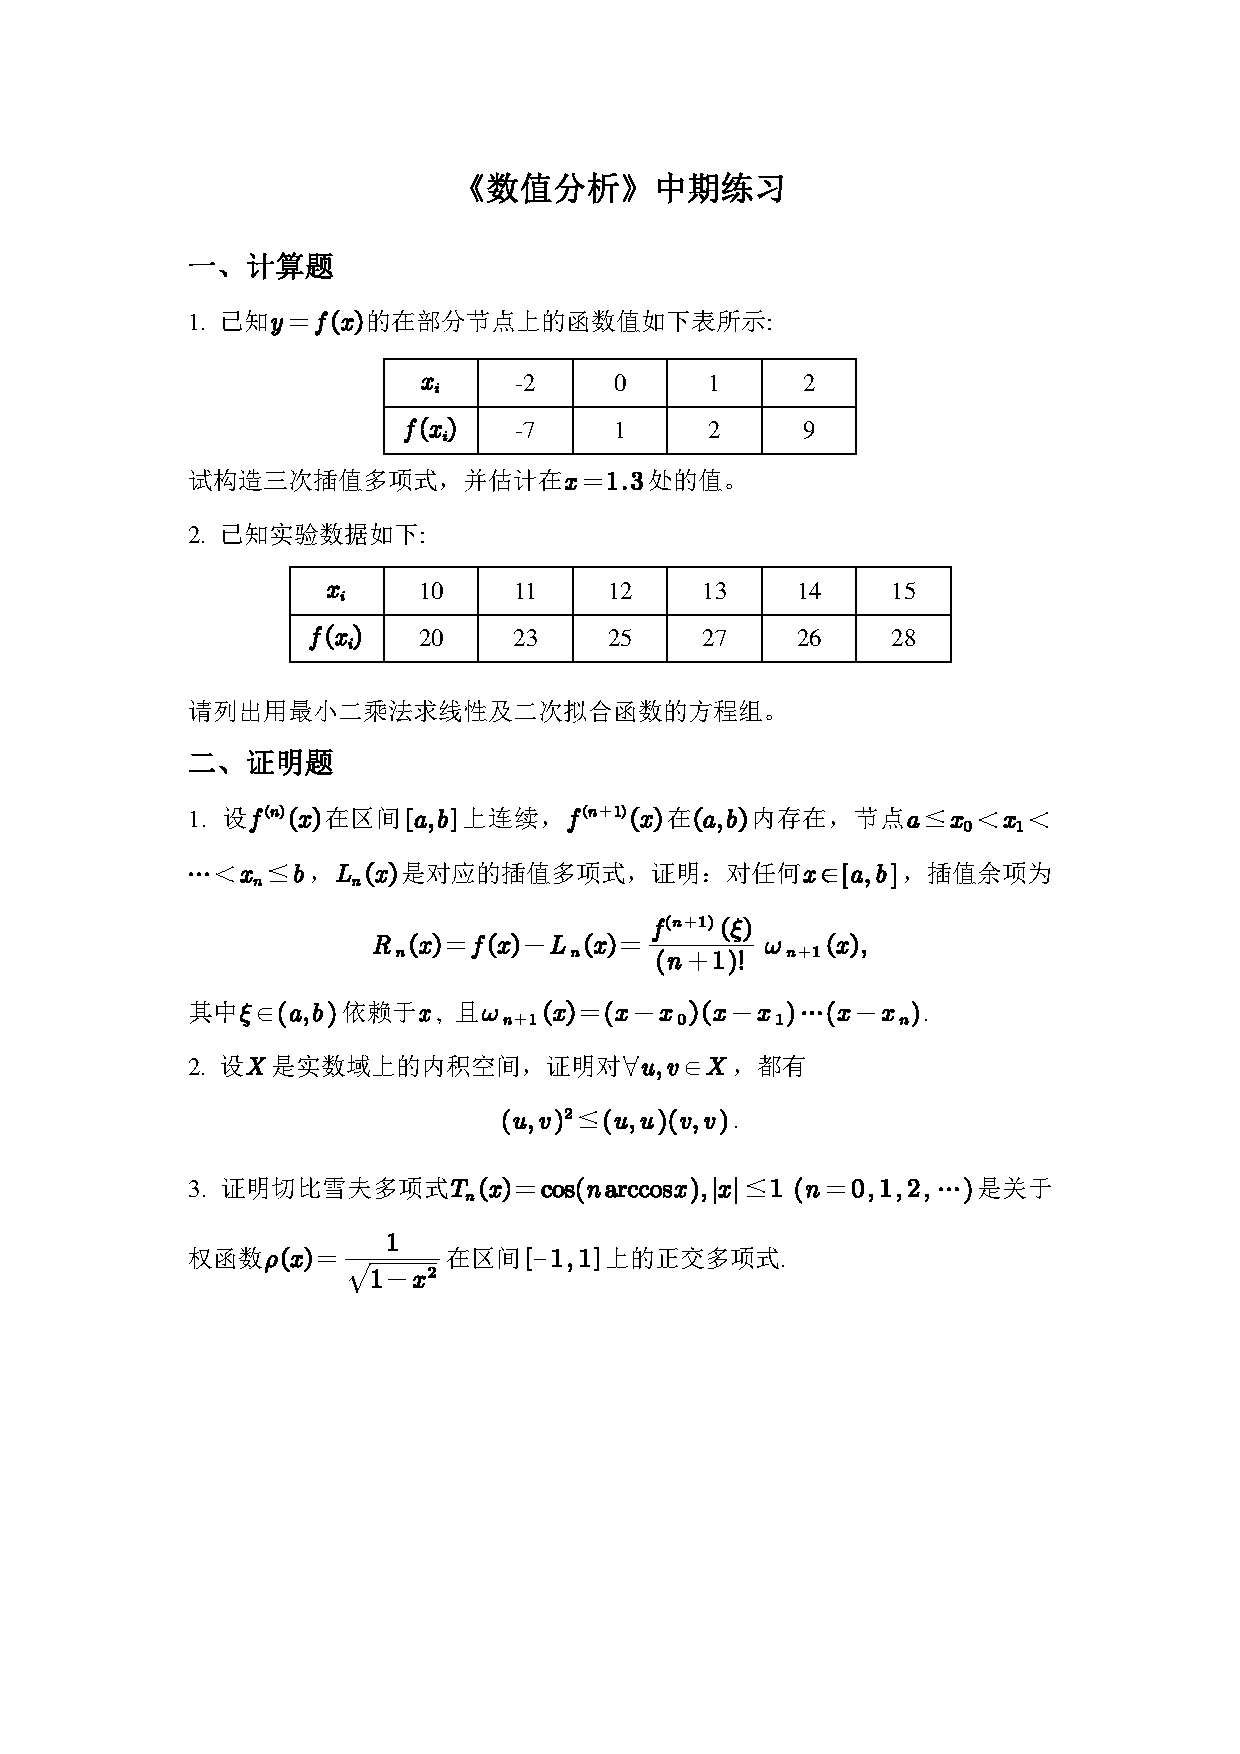
\includepdf{w10/fig.pdf}


	\section{第十一周数值分析实验}
\subsection{牛顿一科特斯积分}
\begin{ex}
	编写牛顿一科特斯积分公式程序, 思路如下:
	
	(1) 对区间 $[a, b]$ 作 $n$ 等份, 确定数值点 $x_k$, 求解被积函数的函数值 $y_k=f\left(x_k\right)$;
	
	(2) 计算第 $k$ 个科特斯系数 $C_k^{(n)}=\frac{(-1)^{n-k}}{n k !(n-k) !} \int_0^n \prod_{\substack{j=0 \\ j \neq k}}^n(t-j) \mathrm{d} t$
	
	(3) 构造牛顿一科特斯积分公式 $\int_a^b f(x) d x=(b-a) \sum_{k=0}^n C_k^{(n)} f\left(x_k\right)$.
	
	(4) 利用 $M A T L A B$ 编写算法实现, 参考函数格式为:
	$$
	I_{\text {out }}=\text { NewtonCotesIntegration }(f, a, b, n)
	$$
\end{ex}
\lstinputlisting[language=matlab]{w11/NewtonCotesIntegration.m}
\subsection*{例子}
\begin{ex}
	利用程序计算下列两个积分
	$$
	I_1=\int_1^9 \sqrt{x} d x \quad \text { 及 } \quad I_2=\int_0^2 \sqrt{4-x^2} \mathrm{~d} x
	$$
	并比较结果
	1. 梯形公式;2. 辛普森公式;3. 科特斯公式.
\end{ex}
\lstinputlisting[language=matlab]{w11/q2.m}
\qa 
% Table generated by Excel2LaTeX from sheet 'Sheet1'
\begin{table}[htbp]
	\centering
	\caption{运行结果}
	\begin{tabular}{l|ccc}
		& \multicolumn{1}{l}{梯形公式} & \multicolumn{1}{l}{Simpson公式} & \multicolumn{1}{l}{柯斯特公式} \\
		\hline
		$I_1$   & 16    & 17.25903 & 17.32644 \\
		$I_2$   & 2     & 2.976068 & 3.090764 \\
	\end{tabular}%
	\label{tab:addlabel11}%
\end{table}%

\begin{ex}
	选择尽可能精确的方法计算下列积分
	$$
	S=a \int_0^{\pi / 2} \sqrt{1-\left(\frac{c}{a}\right)^2 \sin ^2 \theta} d \theta
	$$
	其中
	$$
	\begin{aligned}
		& a=(2 R+H+h) / 2, c=(H-h) / 2, \\
		& R=6371, \quad H=2384, \quad h=439
	\end{aligned}
	$$
\end{ex}
\qa 
\begin{figure}[H]
	\centering
	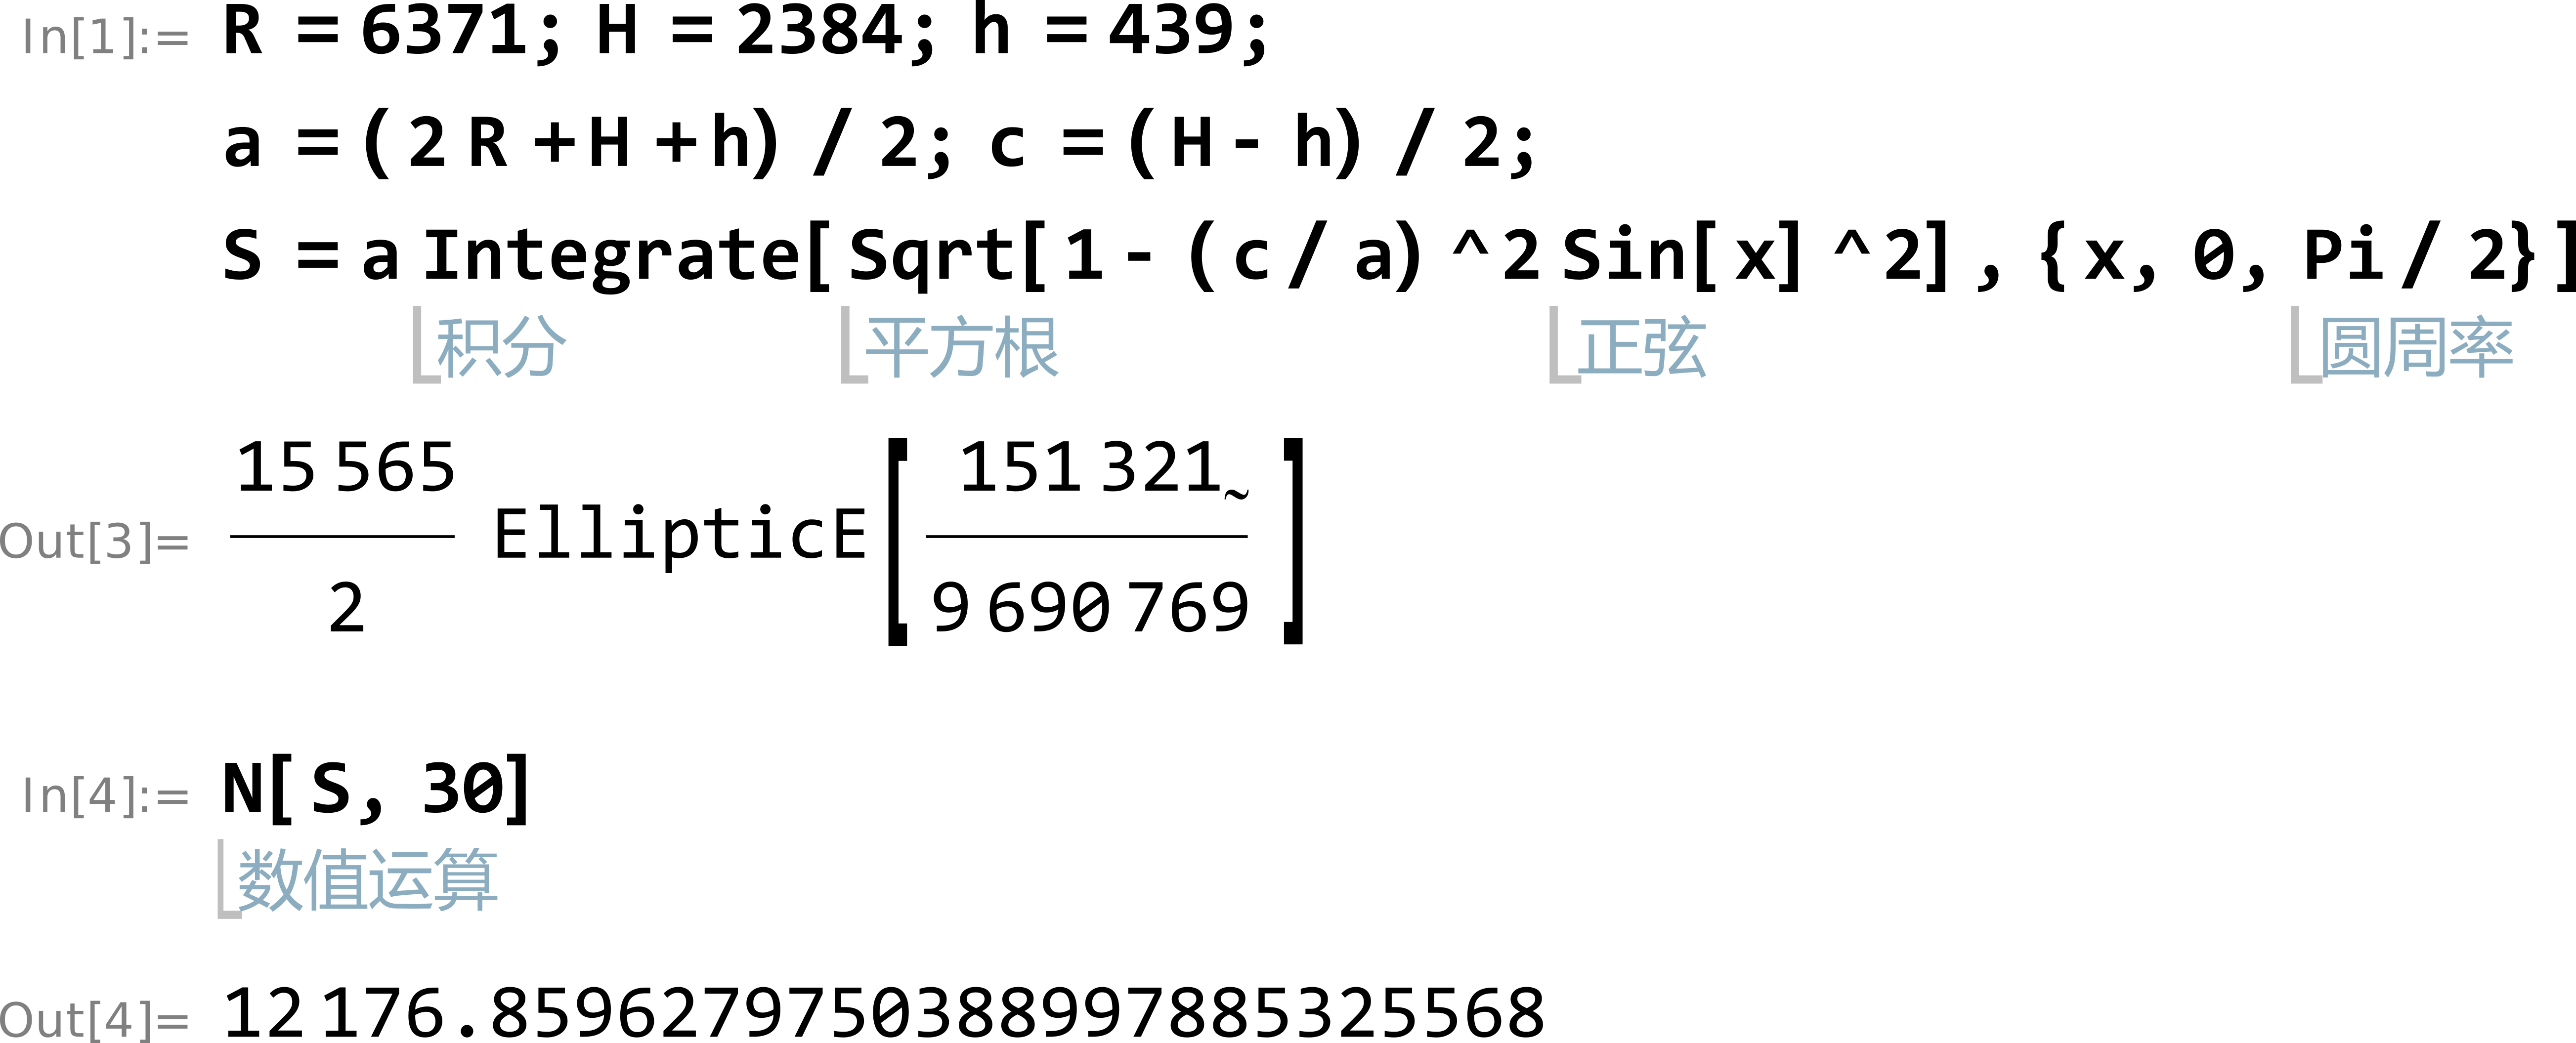
\includegraphics[width = 0.8\linewidth]{w11/fig1.png}
	\caption{Mathematica数值结果}
\end{figure}
\lstinputlisting[language=matlab]{w11/q3.m}
\qa 12176.875336227736163485779741222
\begin{figure}[H]
	\centering
	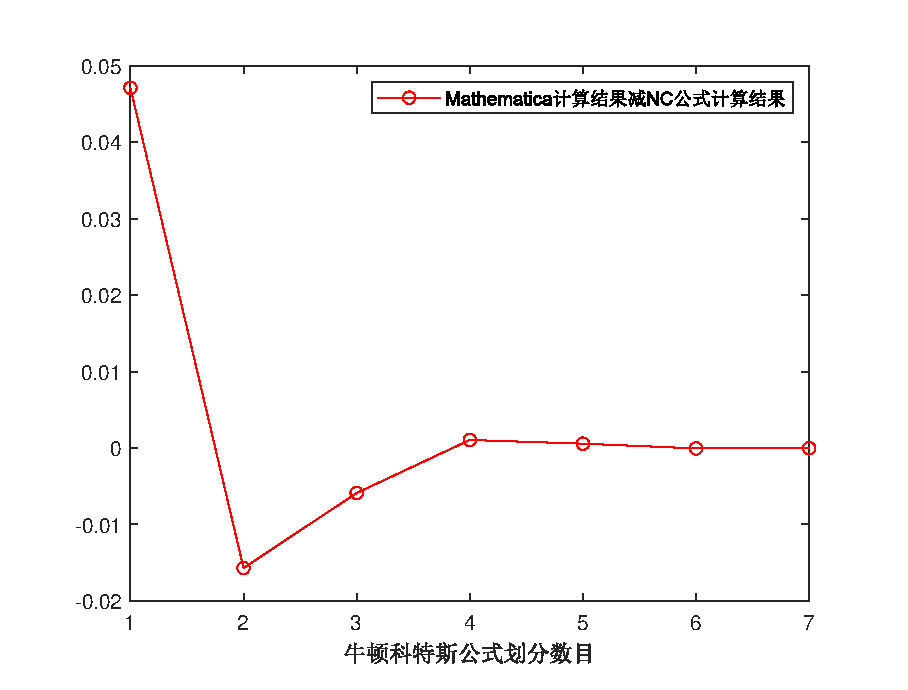
\includegraphics[width = 0.61\linewidth]{w11/fig.eps}
	\caption{结果比较}
\end{figure}


	\section{第十二周数值分析实验}
\subsection{复合梯形公式与复合Simpson公式}
\begin{ex}
	试用复合梯形公式、复合辛普森公式 $(n=4,8,16,32,64)$ 求解积分
	$$
	I=\int_0^5 x^5 e^{-x} \sin x d x
	$$
	
	已知精确值 $-e^{-5}(3660 \cos 5+487.5 \sin 5)-15 \approx-18.8455351153$.
\end{ex}
\lstinputlisting[language=matlab]{w12/q1.m}
\subsection{高斯一勒让德求积公式}
\begin{ex}
	试用$5$个节点的高斯一勒让德求积公式计算上例.
\end{ex}
\lstinputlisting[language=matlab]{w12/q2.m}
\subsection{复合型的高斯一勒让德求积公式}
\begin{ex}
	试用复合型的高斯一勒让德求积公式计算上例, 其中区间做 $n(n=5,10)$ 等份,每个小区间上使用$2$个节点的 $G-L$ 公式.
\end{ex}
\lstinputlisting[language=matlab]{w12/q3.m}
	\section{第十三周数值分析实验}
\subsection{矩阵的LU分解}
\begin{ex}
	实现n阶非奇异矩阵A的LU分解程序,函数格式为:
	$[L,U]=lu\_decomposition(A)$
	并计算P153, 例5.
\end{ex}
\lstinputlisting[language=matlab]{w13/lu_decomposition.m}
\lstinputlisting[language=matlab]{w13/q1.m}
\qa 
\begin{eqnarray*}
	\begin{bmatrix}
		1 & 2 & 3\\
		2 & 5 & 2\\
		3 & 1 & 5
	\end{bmatrix}
	=\begin{bmatrix}
		1&0&0\\
		2&1&0\\
		3&-5&1
	\end{bmatrix}
	\begin{bmatrix}
		1&2&3\\
		0&1&-4\\
		0&0&-24
	\end{bmatrix}
	\Longrightarrow
	\boldsymbol{x}=
	\begin{bmatrix}
		1\\2\\3
	\end{bmatrix}.
\end{eqnarray*}

\subsection{矩阵的Cholesky分解}
\begin{ex}
	实现n阶对称正定矩阵A的Cholesky分解程序,函数格式为:
	
	$L=cholesky\_Factorization (A)$
	并计算P177第9题. (MATLAB自带程序为chol(A)).
\end{ex}
\lstinputlisting[language=matlab]{w13/cholesky_Factorization.m}
\lstinputlisting[language=matlab]{w13/q2.m}
\qa 
\begin{scriptsize}
	\begin{align*}
		\begin{array}{lc}
			\begin{bmatrix}
				1.41421356237310&0&0&0&0\\
				-0.707106781186548&1.22474487139159&0&0&0\\
				0&-0.816496580927726&1.15470053837925&0&0\\
				0&0&-0.866025403784439&1.11803398874990&0\\
				0&0&0&-0.894427190999916&1.09544511501033
			\end{bmatrix}
		\end{array}
	\end{align*}

$\boldsymbol{x}=\left[0.833333333333333,0.666666666666667,0.500000000000000,0.333333333333333,0.166666666666667\right]^T$
\end{scriptsize}
	\section{第十五周数值分析实验}
\subsection{迭代法}
\begin{ex}
设线性方程组 $\left\{\begin{array}{l}8 x_1-3 x_2+2 x_3=20, \\ 4 x_1+11 x_2-x_3=33, \\ 6 x_1+3 x_2+12 x_3=36 .\end{array}\right.$ 精确解是 $x^*=(3,2,1)^T$. 按如下格式求解
$$
\left\{\begin{array}{l}
	x_1{ }^{(k+1)}=\left(3 x_2{ }^{(k)}-2 x_3{ }^{(k)}+20\right) / 8 \\
	x_2{ }^{(k+1)}=\left(-4 x_1{ }^{(k)}+x_3{ }^{(k)}+33\right) / 11 \\
	x_3{ }^{(k+1)}=\left(-6 x_1{ }^{(k)}-3 x_2{ }^{(k)}+36\right) / 12
\end{array}\right.
$$

其中 $x^{(0)}=(0,0,0)^T$. 试给出第 $10,20,100,200,1000$ 次的迭代结果及误差向量的无穷范数.
\end{ex}
\lstinputlisting[language=matlab]{w15/q1.m}
\qa 
% Table generated by Excel2LaTeX from sheet 'Sheet1'
\begin{table}[H]
	\centering
	\caption{运行结果}
	\begin{tabular}{c|ccccc}
		& 10    & 20    & 100   & 200   & 1000 \\
		\hline
		$x_1$    & 2.999982 & 3     & 3     & 3     & 3 \\
		$x_2$    & 1.999978 & 2     & 2     & 2     & 2 \\
		$x_3$    & 1.000016 & 1     & 1     & 1     & 1 \\
		误差向量的无穷范数 & 2.24E-05 & 1.49E-09 & 0     & 0     & 0 \\
	\end{tabular}%
	\label{tab:addlabelw15-1}%
\end{table}%


\begin{ex}
	用高斯一赛德尔迭代法求解练习 1 , 试给出第 $10,20,100,200,1000$ 次的迭代结果及误差向量的无穷范数.
\end{ex}
\subsection{高斯塞德尔迭代法}
\lstinputlisting[language=matlab]{w15/q2.m}
\qa 
% Table generated by Excel2LaTeX from sheet 'Sheet1'
\begin{table}[H]
	\centering
	\caption{运行结果}
	\begin{tabular}{c|ccccc}
		& 10    & 20    & 100   & 200   & 1000 \\
		\hline
		$x_1$    & 3     & 3     & 3     & 3     & 3 \\
		$x_2$    & 2     & 2     & 2     & 2     & 2 \\
		$x_3$    & 1     & 1     & 1     & 1     & 1 \\
		误差向量的无穷范数 & 2.13E-10 & 0     & 0     & 0     & 0 \\
	\end{tabular}%
	\label{tab:addlabel15-2}%
\end{table}%


	\section{第十六周数值分析实验}
\subsection{Jacobi和G-S迭代法}
\begin{ex}
设线性方程组
$$
\left\{\begin{array}{l}
	x_1+2 x_2-2 x_3=1, \\
	x_1+x_2+x_3=1, \\
	2 x_1+2 x_2+x_3=1 .
\end{array}\right.
$$

试编制程序, 列表给出前 10 个迭代向量, 并考察 $J a c o b i$ 和 $G-S$ 迭代法的收玫性.
\end{ex}
\lstinputlisting[language=matlab]{w16/q1.m}
\qa 
% Table generated by Excel2LaTeX from sheet 'Sheet1'
\begin{table}[H]
	\centering
	\caption{运行结果}
	\begin{tabular}{|c|ccccccccccc|}
		\hline
		(Jacobi)n & 0     & 1     & 2     & 3     & 4     & 5     & 6     & 7     & 8     & 9     & 10 \\
		\hline
		$x_1$    & 0     & 1     & 1     & -3    & -3    & -3    & -3    & -3    & -3    & -3    & -3 \\
		$x_2$   & 0     & 1     & -1    & 3     & 3     & 3     & 3     & 3     & 3     & 3     & 3 \\
		$x_3$    & 0     & 1     & -3    & 1     & 1     & 1     & 1     & 1     & 1     & 1     & 1 \\
		\hline\hline
		(G-S)n & 0     & 1     & 2     & 3     & 4     & 5     & 6     & 7     & 8     & 9     & 10 \\
		\hline
		$x_1$    & 0     & 1     & -1    & -11   & -43   & -131  & -355  & -899  & -2179 & -5123 & -11779 \\
		$x_2$    & 0     & 0     & 3     & 15    & 51    & 147   & 387   & 963   & 2307  & 5379  & 12291 \\
		$x_3$    & 0     & -1    & -3    & -7    & -15   & -31   & -63   & -127  & -255  & -511  & -1023 \\
		\hline
	\end{tabular}%
	\label{tab:addlabel-w16-1}%
\end{table}%


\subsection{SOR迭代法}
\begin{ex}
	用 $S O R$ 方法解线性方程组
	$$
	\left(\begin{array}{cccc}
		4 & -1 & -1 & -1 \\
		-1 & 4 & -1 & -1 \\
		-1 & -1 & 4 & -1 \\
		-1 & -1 & -1 & 4
	\end{array}\right)\left(\begin{array}{l}
		x_1 \\
		x_2 \\
		x_3 \\
		x_4
	\end{array}\right)=\left(\begin{array}{l}
		1 \\
		1 \\
		1 \\
		1
	\end{array}\right)
	$$
	
	初值取 $x^{(0)}=(0,0,0,0)^T$, 计算到 $\left\|x^{(k)}-x^{(k-1)}\right\|_{\infty}<10^{-8}$ 停止, 并绘制迭代步数 IT 关于松驰因子 $\omega$ (步长取 0.01$)$ 的图像.
\end{ex}
\lstinputlisting[language=matlab]{w16/q2.m}
\qa
 $\mathbf{x}=\left[0.308641974897860,0.308641979217244,0.308641971803977,0.308641977711201\right]^T.$
\begin{figure}[H]
	\centering
	\subfloat[$0.01\leq \omega\leq 1.99$]{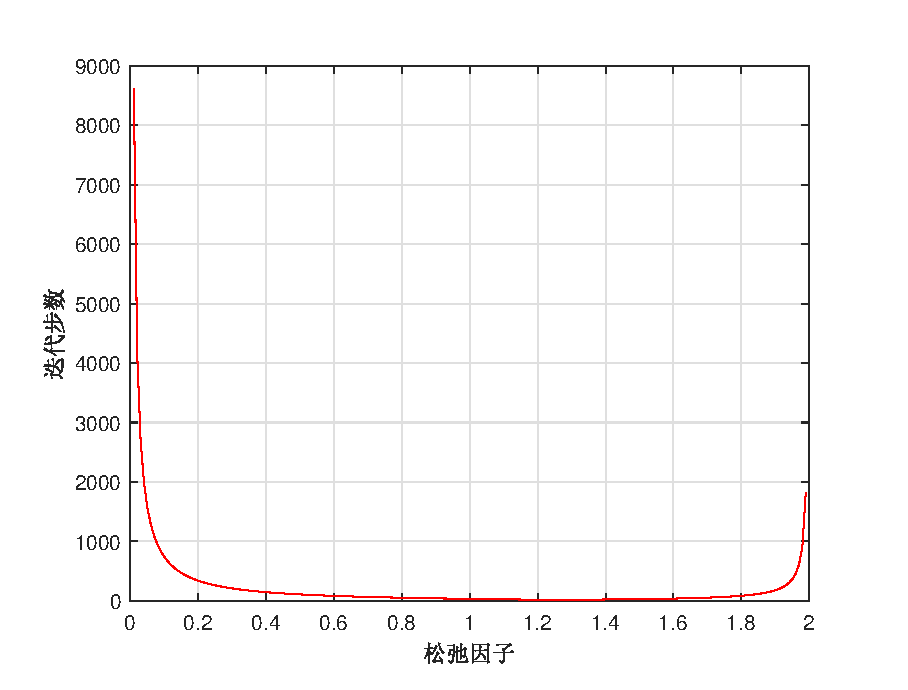
\includegraphics[width = 0.5\linewidth]{w16/q2-l.eps}}
	\hfill
	\subfloat[$0.40\leq \omega\leq 1.80$]{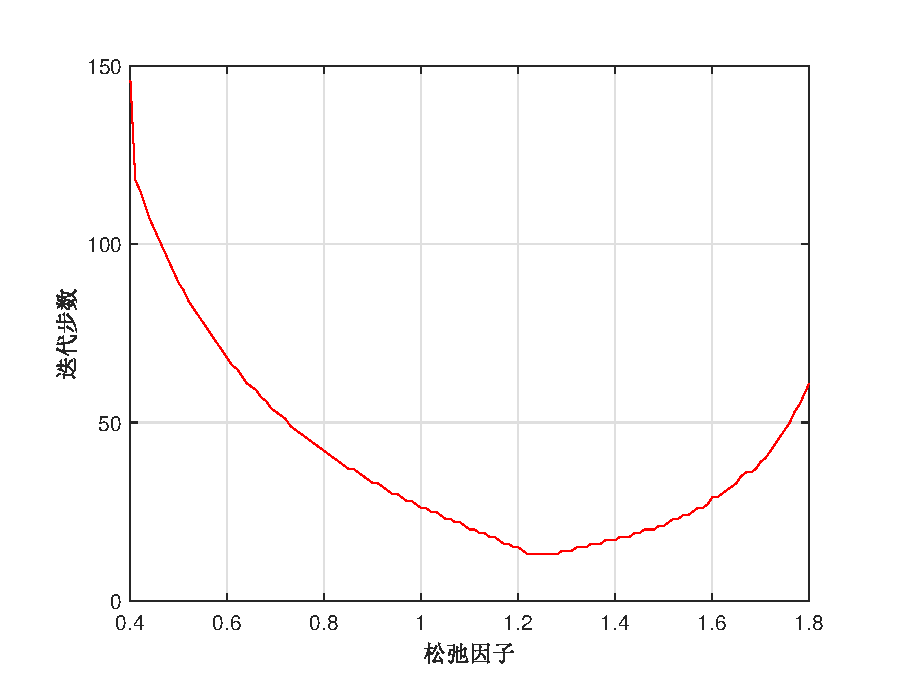
\includegraphics[width = 0.5\linewidth]{w16/q2-s.eps}}
	\caption{迭代步数}
\end{figure}
\subsection{选做题}
\begin{ex}
	已知 $50 \times 50$ 带状方程组, 设初始解向量为 $x^{(0)}=0.01$ ones $(50,1)$, 精度 $\varepsilon=10^{-14}$,试采用 Jacobi 迭代法和 $G-S$ 迭代法求解带状线性方程组满足精度要求的近似解.
	$$
	\left(\begin{array}{llllllll}
		12 & -2 & 1 & & & & & \\
		-2 & 12 & -2 & 1 & & & & \\
		1 & -2 & 12 & -2 & 1 & & & \\
		& 1 & -2 & 12 & -2 & 1 & & \\
		& & \ddots & \ddots & \ddots & \ddots & \ddots & \\
		& & & 1 & -2 & 12 & -2 & 1 \\
		& & & & 1 & -2 & 12 & -2 \\
		& & & & & 1 & -2 & 12
	\end{array}\right)\left(\begin{array}{c}
		x_1 \\
		x_2 \\
		x_3 \\
		x_4 \\
		\vdots \\
		x_{48} \\
		x_{49} \\
		x_{50}
	\end{array}\right)=\left(\begin{array}{c}
		5 \\
		5 \\
		5 \\
		5 \\
		\vdots \\
		5 \\
		5 \\
		5
	\end{array}\right)
	$$
\end{ex}
\lstinputlisting[language=matlab]{w16/q3.m}
\qa 
% Table generated by Excel2LaTeX from sheet 'Sheet1'
\begin{table}[H]
	\centering
	\caption{运行结果}
	\resizebox{1.1\columnwidth}{!}{
	\begin{tabular}{|cccccccc|}
		\hline
		$x_1$ & $x_2$ & $x_3$ & $x_4$ & $x_5$ & $x_6$ & $x_7$ & $x_8$ \\
		0.46379552381655 & 0.537284605199966 & 0.509022924601331 & 0.498221634436174 & 0.498941860239762 & 0.499985351248131 & 0.500088723890136 & 0.500015318846052 \\
		$x_{9}$ & $x_{10}$ & $x_{11}$ & $x_{12}$ & $x_{13}$ & $x_{14}$ & $x_{15}$ & $x_{16}$ \\
		0.499994793266975 & 0.499997856913468 & 0.500000108425199 & 0.500000201576687 & 0.500000022610945 & 0.499999986238572 & 0.499999995873979 & 0.500000000530294 \\
		$x_{17}$ & $x_{18}$ & $x_{19}$ & $x_{20}$ & $x_{21}$ & $x_{22}$ & $x_{23}$ & $x_{24}$ \\
		0.500000000439039 & 0.500000000023939 & 0.499999999966017 & 0.499999999992557 & 0.500000000001741 & 0.500000000000922 & 0.499999999999990 & 0.499999999999923 \\
		$x_{25}$ & $x_{26}$ & $x_{27}$ & $x_{28}$ & $x_{29}$ & $x_{30}$ & $x_{31}$ & $x_{32}$ \\
		0.499999999999998 & 0.499999999999987 & 0.499999999999921 & 0.500000000000001 & 0.500000000000915 & 0.500000000001741 & 0.499999999992558 & 0.499999999966019 \\
		$x_{33}$ & $x_{34}$ & $x_{35}$ & $x_{36}$ & $x_{37}$ & $x_{38}$ & $x_{39}$ & $x_{40}$ \\
		0.500000000023937 & 0.500000000439038 & 0.500000000530295 & 0.499999995873980 & 0.499999986238572 & 0.500000022610945 & 0.500000201576688 & 0.500000108425199 \\
		$x_{41}$ & $x_{42}$ & $x_{43}$ & $x_{44}$ & $x_{45}$ & $x_{46}$ & $x_{47}$ & $x_{48}$ \\
		0.499997856913467 & 0.499994793266975 & 0.500015318846052 & 0.500088723890136 & 0.499985351248131 & 0.498941860239762 & 0.498221634436174 & 0.509022924601331 \\
		$x_{49}$ & $x_{50}$ &       &       &       &       &       &  \\
		0.537284605199966 & 0.463795523816550 &       &       &       &       &       &  \\
		\hline
	\end{tabular}%
	}
	\label{tab:addlabel-w16-q3}%
\end{table}%


	\ClearWallPaper
	%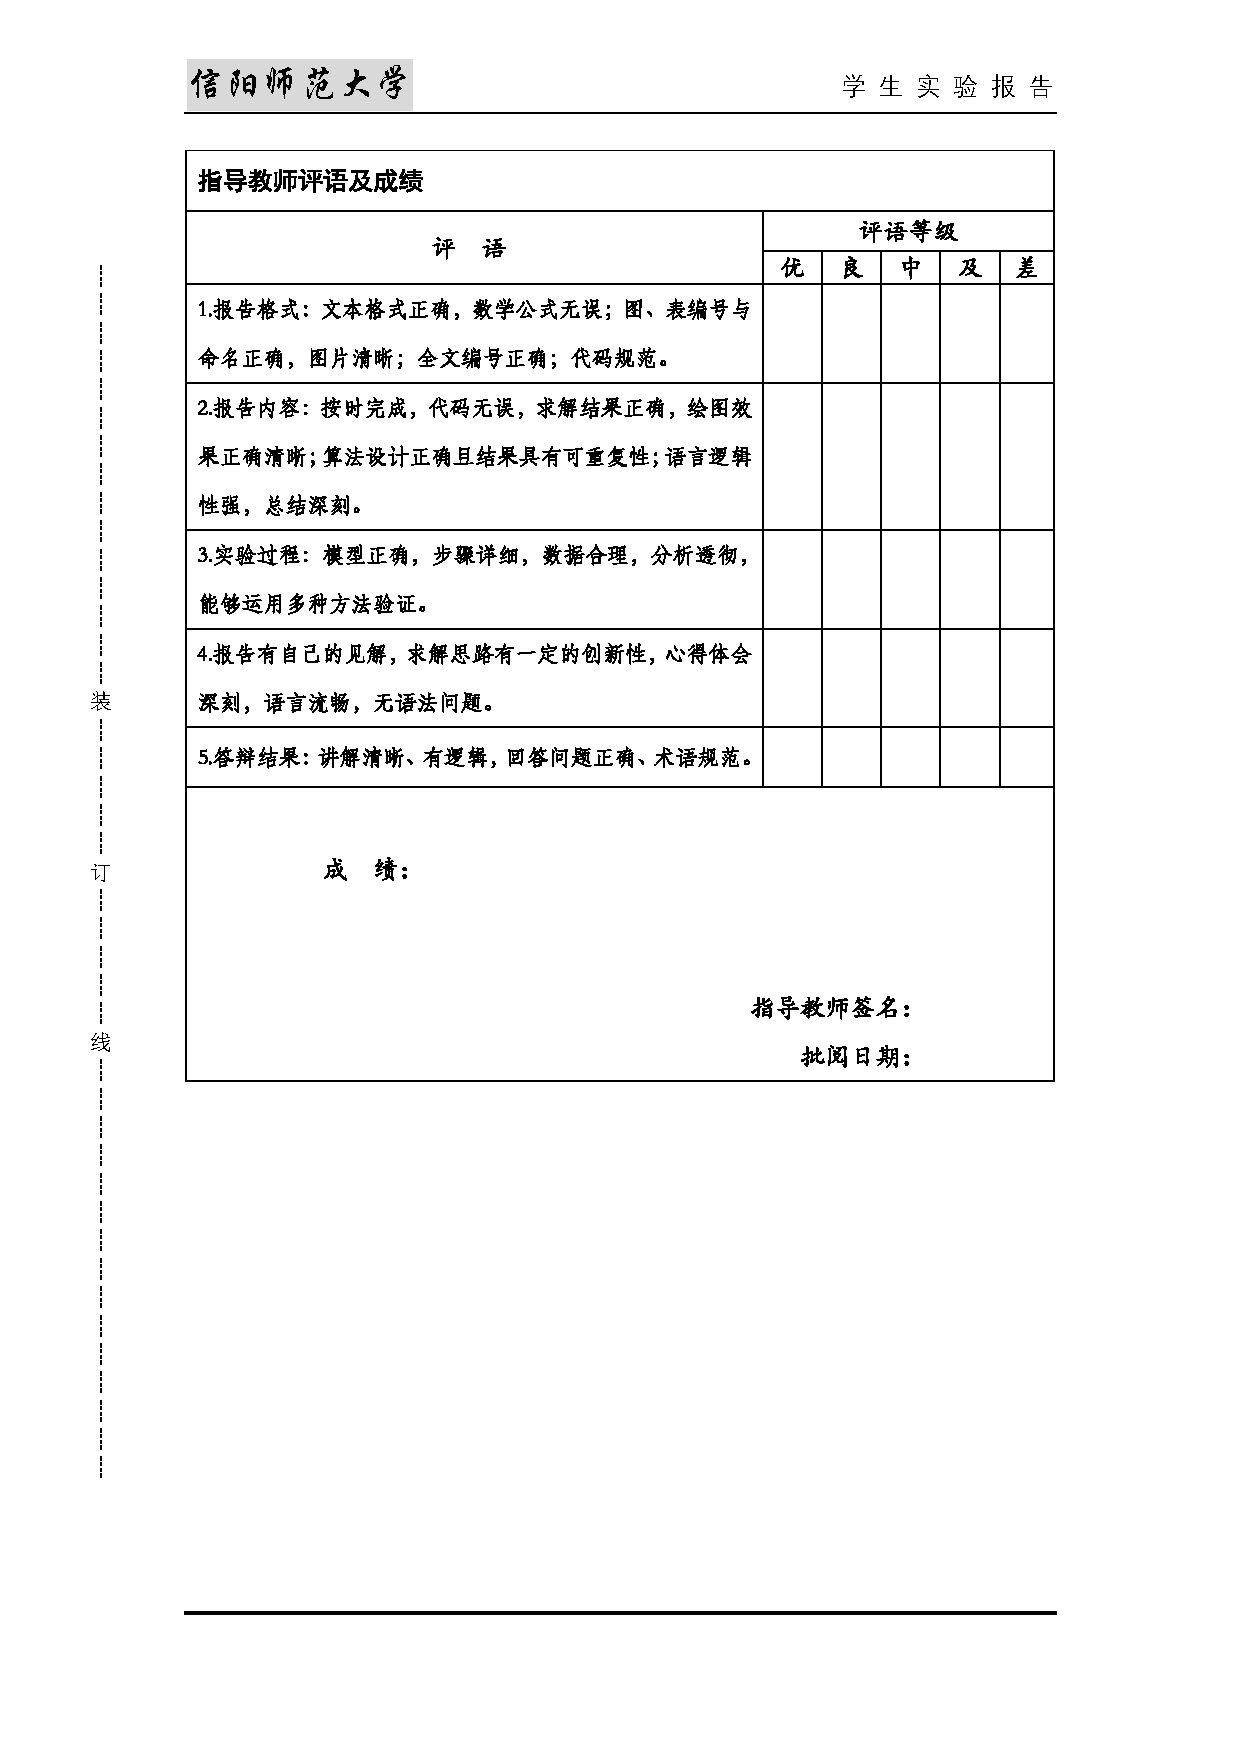
\includepdf[]{pageset/lastpage.pdf}
\end{document}